\chapter{启动操作系统}\label{ch_boot}

\section{本章概要}

\paragraph{一句话描述}
站在操作系统的最底层,了解操作系统的启动,与物理硬件:CPU,内存和多种外设实现“零距离”接触,看到它们并管理它们!

\paragraph{概述}

其实这一章的内容与操作系统原理相关的部分较少,与计算机体系结构的细节相关的部分较多。但这些内容对写一个操作系统关系较大,要知道操作系统是直接与硬件打交道的软件,所以它需要``知道''需要硬件细节,才能更好地控制硬件。另一方面,部分内容涉及到操作系统的重要抽象--中断类异常,能够充分理解中断类异常为以后进一步了解进程切换、上下文切换等概念会很有帮助。

\paragraph{本章收获的知识}

\begin{itemize}
	\item
	与操作系统原理相关
	\item
	I/O设备管理:涉及程序循环检测方式和中断启动方式、I/O地址空间
	\item
	内存管理:基于分段机制的内存管理
	\item
	异常处理:涉及中断、故障和陷阱
	\item
	特权级:内核态和用户态
	\item
	计算机系统和编程
	\item
	硬件	
	\begin{itemize}
		\item
		计算机从加电到加载操作系统内核的整个过程
		\item
		OS内核在内存中的布局
		\item
		串口访问、时钟访问
	\end{itemize}
	\item
	软件	
	\begin{itemize}
		\item
		ELF执行文件格式
		\item
		栈的实现并实现函数调用栈跟踪函数
		\item
		调试操作系统
	\end{itemize}
\end{itemize}

\paragraph{本章涉及的实验}

本章的实验内容涉及的是写一个bootloader能够启动一个操作系统--ucore。在完成bootloader的过程中,逐渐增加bootloader和ucore的能力,涉及CPU的模式切换、解析ELF执行文件格式等,这对于理解操作系统的加载过程以及在操作系统在内存中的位置、内存管理、用户态与内核态的区别等有帮助。而相关project中bootloader和操作系统本身的字符显示的I/O处理、读硬盘数据的I/O处理、键盘/时钟的中断处理等内容,则是操作系统原理中一般在靠后位置提到的设备管理的实际体现。纵观操作系统的发展史,从早期到现在的操作系统主要功能之一就是完成繁琐的I/O处理,给上层应用提供比较简洁的I/O服务,屏蔽硬件处理的复杂性。这也是操作系统的虚拟机功能的体现。另外,本章还介绍了对硬件模拟器的使用,对操作系统的panic处理和远程debug功能的支持,这样有助于读者能够方便地分析操作系统中的错误和调试操作系统。由于本章涉及的硬件知识较多,无疑增大了读者的阅读难度,需要读者在结合阅读本章并实际动手实验来进行深入理解。

读者通过阅读本章的内容并动手实践相关的4个实验项目:

\begin{itemize}
	\item
	proj1:能够显示字符的bootloader
	\item
	proj2/3:可读ELF格式文件的bootloader和显示字符的ucore
	\item
	proj4:可管理中断和处理基于中断的键盘/时钟的ucore
\end{itemize}





\section{显示字符的toy
bootloader}\label{ux663eux793aux5b57ux7b26ux7684toy-bootloader}

\subsection{实验目标}\label{ux5b9eux9a8cux76eeux6807}

操作系统是一个软件,也需要通过某种手段加载并运行它。在这里我们将通过另外一个更加简单的软件-bootloader来完成这些工作。为此,我们需要完成一个能够切换到x86的保护模式并显示字符的bootloader,为将来启动操作系统做准备。proj1提供了一个非常小的bootloader,整个bootloader的大小小于512个字节,这样才能放到硬盘的主引导扇区中。
\textgreater{} 这里对x86的保护模式不必太在意,后续会进一步讲解

通过分析和实现这个bootloader,读者可以了解到: * 与操作系统原理相关 *
I/O设备管理:设备管理的基本概念,涉及简单的信息输出 *
内存管理:基于分段机制的存储管理,x86的实模式/保护模式以及切换到保护模式的方法
* 计算机系统和编程 * 硬件 * PC加电后启动bootloader的过程 *
通过串口/并口/CGA输出字符的方法 * 软件 * bootloader的文件组成 *
编译运行bootloader的过程 * 调试bootloader的方法 *
在汇编级了解栈的结构和处理过程

\subsection{proj1概述}\label{proj1ux6982ux8ff0}

\subsubsection{实现描述}\label{ux5b9eux73b0ux63cfux8ff0}

proj1实现了一个简单的bootloader,主要完成的功能是初始化寄存器内容,完成实模式到保护模式的转换,在保护模式下通过PIO方式控制串口、并口和CGA等进行字符串输出。

\subsubsection{项目组成}\label{ux9879ux76eeux7ec4ux6210}

{[}要点(非OSP):bootloader的编译生成过程{]}
lab1中包含的第一个工程小例子是proj1:一个可以切换到保护模式并显示字符串的bootloader。proj1的整体目录结构如下所示:

\begin{lstlisting}
    proj1 /
    |-- boot
    |   |-- asm.h
    |   |-- bootasm.S
    |   `-- bootmain.c
    |-- libs
    |   |-- types.h
    |   `-- x86.h
    |-- Makefile
    `-- tools
        |-- function.mk
        |-- gdbinit
        `-- sign.c

    3 directories, 9 files
\end{lstlisting}

其中一些比较重要的文件说明如下: * bootasm.S
:定义并实现了bootloader最先执行的函数start,此函数进行了一定的初始化,完成了从实模式到保护模式的转换,并调用bootmain.c中的bootmain函数。
*
bootmain.c:定义并实现了bootmain函数实现了通过屏幕、串口和并口显示字符串。
*
asm.h:是bootasm.S汇编文件所需要的头文件,主要是一些与X86保护模式的段访问方式相关的宏定义。
* types.h:包含一些无符号整型的缩写定义。 * x86.h:一些用GNU
C嵌入式汇编实现的C函数(由于使用了inline关键字,所以可以理解为宏)。 *
Makefile和function.mk:指导make完成整个软件项目的编译,清除等工作。 *
sign.c:一个C语言小程序,是辅助工具,用于生成一个符合规范的硬盘主引导扇区。
* gdbinit:用于gdb远程调试的初始命令脚本

从中,我们可以看出bootloader主要由bootasm.S和bootmain.c组成,当你完成编译后,你会发现这个bootloader只有区区的3百多字节。下面是编译运行bootloader的过程。

\begin{quote}
【提示】bootloader是一个超小的系统软件,在功能上与我们一般的应用软件不同,主要用于硬件简单初始化和加载运行操作系统。在编写bootloader的时候,需要了解它所处的硬件环境(比如它在内存中的起始地址,它的储存空间的位置和大小限制等)。而这些是编写应用软件不太需要了解的,因为操作系统和编译器帮助应用软件考虑了这些问题。
\end{quote}

\subsubsection{编译运行}\label{ux7f16ux8bd1ux8fd0ux884c}

\textbf{【实验 编译运行bootloader】}

在proj1下执行make,在proj1/bin目录下可生成一个ucore.img。ucore.img是一个包含了bootloader或OS的硬盘镜像,通过执行如下命令可在硬件虚拟环境
qemu中运行bootloader或OS:

\begin{lstlisting}
  make                     //生成bootloader和对应的主引导扇区
  make qemu          //通过qemu硬件模拟器来运行bootloader
  make clean          //清除生成的临时文件,bootloader和对应的主引导扇区
\end{lstlisting}

%\begin{figure}[htbp]
%\centering
%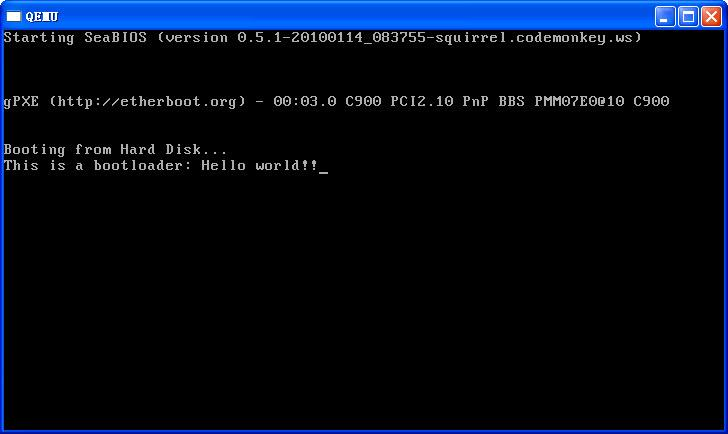
\includegraphics{figures/qemu_cha1.jpg}
%\caption{qemu\_img}
%\end{figure}

我们除了需要了解bootloader的功能外,还需要进一步了解bootloader的编译链接和最终执行码的生成过程,从而能够清楚生成的代码是否是我们所期望的。proj1中的Makefile是一个配置脚本,make软件工具能够通过Makefile完成管理bootloader的C/ASM代码生成执行码的整个过程。Makefile的内容比较复杂,不过读者在前期只需会执行make
{[}参数{]}来生成代码和清除代码即可。对于本实验的make的执行过程如下所示:

\begin{lstlisting}
    1. gcc -O2 -o tools/sign tools/sign.c
    2. i386-elf-gcc -fno-builtin -Wall -MD -ggdb -m32 -fno-stack-protector -O -nostdinc -Iinclude -Iinclude/x86 -c bootloader/bootmain.c -o obj/bootmain.o
    3. i386-elf-gcc -fno-builtin -Wall -MD -ggdb -m32 -fno-stack-protector -nostdinc -Iinclude -Iinclude/x86 -c bootloader/bootasm.S -o obj/bootasm.o
    4. i386-elf-ld  -N -e start -Ttext 0x7C00 -o obj/bootblock.o obj/bootasm.o obj/bootmain.o
    5. i386-elf-objdump -S obj/bootblock.o > obj/bootblock.asm
    6. i386-elf-objcopy -S -O binary obj/bootblock.o obj/bootblock.out
    7. sign.exe obj/bootblock.out obj/bootblock
       obj/bootblock.out size: 380 bytes
       build 512 bytes boot sector: obj/bootblock success!
    8. dd if=/dev/zero of=obj/ucore.img count=10000
       10000+0 records in
       10000+0 records out
       5120000 bytes (5.1 MB) copied, 0.509 s, 10.1 MB/s
    9. dd if=obj/bootblock of=obj/ucore.img conv=notrunc
       1+0 records in
       1+0 records out
       512 bytes (512 B) copied, 0.011 s, 46.5 kB/s
\end{lstlisting}

\textbf{这9步的含义是:}

\begin{lstlisting}
1. 编译生成sign执行程序,用于生成一个符合规范的硬盘主引导扇区;
2. 用gcc编译器编译bootmain.c,生成ELF格式的目标文件bootmain.o;
3. 用gas汇编器(gcc只是一个包装)编译bootasm.S,生成ELF格式的目标文件bootasm.o;
4. 用ld链接器把bootmain.o和bootasm.o链接在一起,形成生成ELF格式的执行文件bootblock.o;
5. 目标文件信息导出工具objdump反汇编bootblock.o,生成bootblock.asm,通过查看bootlock.asm内容,可以了解bootloader的实际执行代码;
6. 文件格式转换和拷贝工具objcopy把ELF格式的执行文件bootblock.o转换成binary格式的执行文件bootblock.out;
7. 通过sign执行程序,把bootblock.out(本身大小需要小于510字节)扩展到512字节,形成一个符合规范的硬盘主引导扇区bootblock;
8. 设备级转换与拷贝工具dd生成一个内容都为“0”的磁盘文件ucore.img;
9. 设备级转换与拷贝工具dd进一步把bootblock覆盖到ucore.img的前512个字节空间中,这样就可以把ucore.img作为一个可启动的硬盘被硬件模拟器qemu使用。
\end{lstlisting}

如果需要了解Makefile中的内容,需要进一步看看附录``ucore实验中的常用工具''一节。

\section{【背景】Intel
80386加电后启动过程}\label{ux80ccux666fintel-80386ux52a0ux7535ux540eux542fux52a8ux8fc7ux7a0b}

\textbf{【要点(非OSP):80836物理内存地址空间】}

\textbf{【要点(非OSP):80836加电后的第一条指令位】}

大家一般都知道bootloader负责启动操作系统,但bootloader自身是被谁加载并启动的呢?为了追根溯源,我们需要了解当计算机加电启动后,到底发生了什么事情。

对于绝大多数计算机系统而言,操作系统和应用软件是存放在磁盘(硬盘/软盘)、光盘、EPROM、ROM、Flash等可在掉电后继续保存数据的存储介质上。当计算机加电后,一般不直接执行操作系统,而是一开始会到一个特定的地址开始执行指令,这个特定的地址存放了系统初始化软件,通过执行系统初始化软件(可固化在ROM或Flash中,也称firmware,固件)完成基本I/O初始化和引导加载操作系统的功能。简单地说,系统初始化软件就是在操作系统内核运行之前运行的一段小软件。通过这段小软件的基本I/O初始化部分,我们可以初始化硬件设备、建立系统的内存空间映射图,从而将系统的软硬件环境带到一个合适的状态,以便为最终调用操作系统内核准备好正确的环境。最终系统初始化软件的引导加载部分把操作系统内核映像加载到RAM中,并将系统控制权传递给它。

对于基于Intel 80386的计算机而言,其中的系统初始化软件由BIOS (Basic Input
Output
System,即基本输入/输出系统,其本质是一个固化在主板Flash/CMOS上的软件)和位于软盘/硬盘引导扇区中的OS
Boot
Loader(在ucore中的bootasm.S和bootmain.c)一起组成。BIOS实际上是被固化在计算机ROM(只读存储器)芯片上的一个特殊的软件,为上层软件提供最底层的、最直接的硬件控制与支持。

以基于Intel
80386的计算机为例,计算机加电后,整个物理地址空间如下图所示:

%\begin{figure}[htbp]
%\centering
%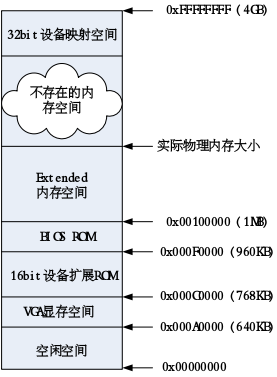
\includegraphics{figures/3.13.1.png}
%\caption{3.13.1.png}
%\end{figure}

图2-1 基于Intel 80386的计算机物理地址空间

处理器处于实模式状态(在86386中,段机制一直存在,可进一步参考2.1.5
【背景】理解保护模式和分段机制),从物理地址0xFFFFFFF0开始执行。初始化状态的CS和EIP确定了处理器的初始执行地址,此时CS中可见部分-选择子(selector)的值为0xF000,而其不可见部分-基地址(base)的值为0xFFFF0000;EIP的值是0xFFF0,这样实际的线性地址(由于没有启动也机制,所以线性地址就是物理地址)为CS.base+EIP=0xFFFFFFF0。在0xFFFFFFF0这里只是存放了一条跳转指令,通过跳转指令跳到BIOS例行程序起始点。更详细的解释可以参考文献{[}1{]}的第九章的9.1节``INITIALIZATION
OVERVIEW''。另外,我们可以通过硬件模拟器qemu来进一步认识上述结果。

\subsubsection{实验2-1:通过qemu了解Intel
80386启动后的CS和EIP值,并分析第一条指令的内容}\label{ux5b9eux9a8c2-1ux901aux8fc7qemuux4e86ux89e3intel-80386ux542fux52a8ux540eux7684csux548ceipux503cux5e76ux5206ux6790ux7b2cux4e00ux6761ux6307ux4ee4ux7684ux5185ux5bb9}

\begin{enumerate}
\def\labelenumi{\arabic{enumi}.}
\item
  启动qemu并让其停到执行第一条指令前,这需要增加一个参数''-S'' qemu --S
\item
  这是qemu会弹出一个没有任何显示内容的图形窗口,显示如下:
\end{enumerate}

%\begin{figure}[htbp]
%\centering
%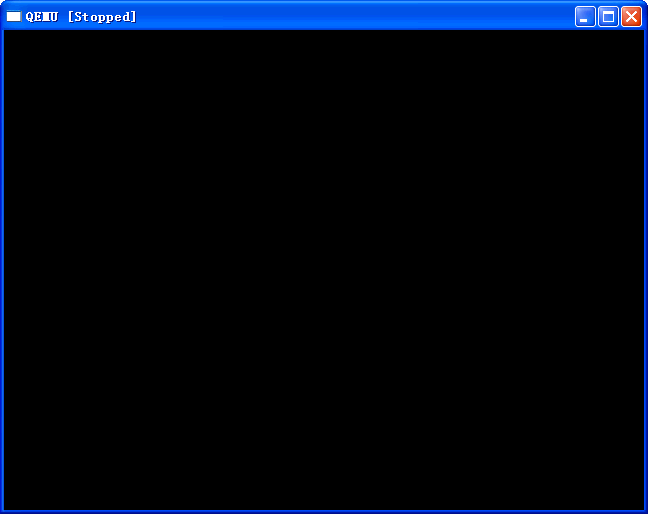
\includegraphics{figures/3.13.2.png}
%\caption{3.13.2.png}
%\end{figure}

\begin{enumerate}
\def\labelenumi{\arabic{enumi}.}
\setcounter{enumi}{2}
\item
  然后通过按''Ctrl+Alt+2''进入qemu的monitor界面,为了了解80386此时的寄存器内容,在monitor界面下输入命令
  ``info registers''
\end{enumerate}

%\begin{figure}[htbp]
%\centering
%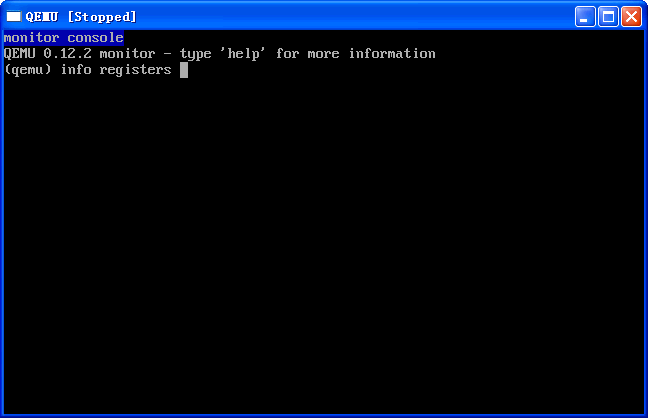
\includegraphics{figures/3.13.3.png}
%\caption{3.13.3.png}
%\end{figure}

\begin{enumerate}
\def\labelenumi{\arabic{enumi}.}
\setcounter{enumi}{3}
\item
  可获得intel 80386启动后执行第一条指令前的寄存器内容,如下图所示
\end{enumerate}

%\begin{figure}[htbp]
%\centering
%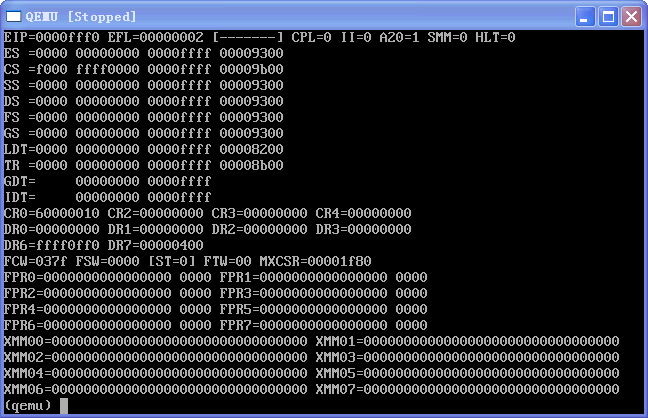
\includegraphics{figures/3.13.4.png}
%\caption{3.13.4.png}
%\end{figure}

从上图中,我们可以看到EIP=0xfff0,CS的selector=0xf000,CS的base=0xfff0000。

BIOS做完计算机硬件自检和初始化后,会选择一个启动设备(例如软盘、硬盘、光盘等),并且读取该设备的第一扇区(即主引导扇区或启动扇区)到内存一个特定的地址0x7c00处,然后CPU控制权会转移到那个地址继续执行。至此BIOS的初始化工作做完了,进一步的工作交给了ucore的bootloader;ucore的bootloader会完成处理器从实模式到保护模式的转换,并从硬盘上读取并加载ucore。其大致流程如下图所示:

%\begin{figure}[htbp]
%\centering
%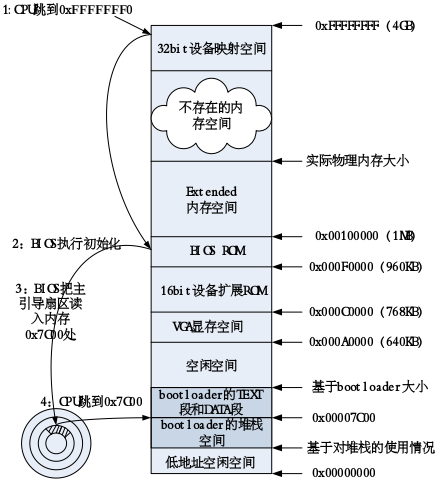
\includegraphics{figures/3.13.5.png}
%\caption{3.13.5.png}
%\end{figure}

图2-2 Intel80386启动过程

\section{【背景】设备管理:理解设备访问机制}\label{ux80ccux666fux8bbeux5907ux7ba1ux7406ux7406ux89e3ux8bbeux5907ux8bbfux95eeux673aux5236}

在本章涉及的bootloader和ucore都需要对I/O设备进行访问,比如通过串口、并口和CGA显示器显示字符串,读取硬盘数据,处理时钟中断等,已经需要读者用到操作系统的I/O设备管理知识了。为此,我们需要操作系统的设备管理进行一个简要描述。

在计算机系统中,操作系统需要管理各种设备,即给它们发送控制命令、捕获中断、错误处理等;为此专门设置了一个子系统:设备管理子系统来完成这些琐碎的工作。同时设备管理子系统还需要提供一个简单易用的统一接口,并尽可能地使其他内核功能组件或应用可通过这个统一接口访问所有的设备,即实现与设备的无关性。比如在proj1中,bootloader提供了一个显示字符的函数接口cons\_putc(位于bootmain.c中),在proj3中的提供了一个显示格式化信息的函数接口cprintf(位于printf.c中),这样操作系统的其他功能组件就可以直接使用这些简单易用的接口来输出信息,而不是通过繁琐的I/O命令与具体的设备打交道。cprintf的实现相对复杂,用到C语言的可变列表参数等,大家只要把它的功能理解为C语言应用库中的printf的简化版即可,并掌握最后是如何通过调用cons\_putc函数完成具体的I/O字符输出。

接下来,我们将从操作系统概念的角度对I/O设备组成、控制设备的方式进行阐述,并进一步对实验中所使用的基于Programmed
I/O (PIO)方式访问并口、CGA和硬盘进行具体分析。

\subsection{硬件设备简介}\label{ux786cux4ef6ux8bbeux5907ux7b80ux4ecb}

对于硬件设备而言,操作系统所关心的并不是硬件自身的设计,而是如何来对它进行控制,即该硬件所接受的控制命令、所完成的功能,以及所返回的出错。所以在设计操作系统的设备管理子系统时,需要了解计算机系统中I/O总线上连接的I/O控制器(比如PC机中的CGA控制器、串口控制器、并口控制器、时钟控制器8254,中断控制器8259等)。

I/O控制器在物理上包含三个层次:I/O地址空间、I/O接口和设备控制器。每个连接到I/O总线上的设备都有自己的I/O地址空间(即I/O端口),这也是CPU可以直接访问的地址。在
PC机中,支持基于I/O的I/O地址空间(通过IN/OUT这类的I/O访问指令访问),也支持基于内存的I/O地址空间(通过MOV等访存指令访问)。这些I/O访问请求通过I/O总线传递给I/O接口。

I/O接口是处于一组I/O端口和对应的设备控制器之间的一种硬件电路。它将I/O访问请求中的特定值转换成设备所需要的命令和数据;并且检测设备的状态变化,及时将各种状态信息写回到特定I/O地址空间,供操作系统通过I/O访问指令来访问。I/O接口包括键盘接口、图形接口、磁盘接口、总线鼠标、网络接口、括并口、串口、通用串行总线、PCMCIA接口和SCSI接口等。

设备控制器并不是所有I/O设备所必须的,只有少数复杂的设备才需要。它负责解释从I/O接口接收到的高级命令,并将其以适当的方式发送到I/O设备;并且对I/O设备发送的消息进行解释并修改I/O端口的状态寄存器。典型的设备控制器就是磁盘控制器,它将CPU发送过来的读写数据指令转换成底层的磁盘操作。

\subsection{控制设备的方式}\label{ux63a7ux5236ux8bbeux5907ux7684ux65b9ux5f0f}

操作系统对硬件设备的控制方式主要与三种:程序循环检测方式(Programmed
I/O,简称PIO)、中断驱动方式(Interrupt-driven I/O)、直接内存访问方式(DMA,
Direct Memory Access)。

在本章的proj1实验中,bootloader需要显示字符串,就是采用相对简单的PIO方式。PIO方式是一种通过CPU执行I/O端口指令来进行数据读写的数据交换模式,被广泛应用于硬盘、光驱等设备的基础传输模式中。这种I/O访问方式使用CPU
I/O端口指令来传送所有的命令、状态和数据,需要处理器全程参与,效率较低,但编程很简单。后面讲到的中断方式和直接内存访问(Direct
Memory Access,DMA)方式将更加高效。

对于程序循环检测方式而言,其控制方式体现在执行过程中通过不断地检测I/O设备的当前状态,来控制I/O操作。具体而言,在进行I/O操作之前,要循环地检测设备是否就绪;在I/O操作进行之中,要循环地检测设备是否已完成;在I/O操作完成之后,还要把输入的数据保存到内存(输入操作)。从硬件的角度来说,控制I/O的所有工作均由CPU来完成。所以此方式也称为繁忙等待方式(busy
waiting)或轮询方式(polling)。其缺点是在进行I/O操作时,一直占用CPU时间。

中断驱动方式的基本思路是用户任务通过系统调用函数来发起I/O操作。执行系统调用后会阻塞该任务,调度其他的任务使用CPU。在I/O操作完成时,设备向CPU发出中断,然后在中断服务例程中做进一步的处理。在中断驱动方式下,数据的每次读写还是通过CPU来完成。但是当I/O设备在进行数据处理时,CPU不必等待,可以继续执行其他的任务。采用这种方式可提供CPU利用率。编程方面,要考虑异步特性,相对麻烦一些。

使用DMA的控制方式,首先需要有DMA控制器。该控制器可集成在设备控制器中,也可集成在主板上。DMA控制器可以直接去访问系统总线,它能代替CPU指挥I/O设备与内存之间的数据传送,在执行完毕后再通知CPU。这种方式可大大减少CPU的执行开销,适合大数据量的设备数据传送。在编程方面,需要对DMA进行编程和异步中断编程,相对更加复杂一些。

\subsection{串口(serial
port)访问控制}\label{ux4e32ux53e3serial-portux8bbfux95eeux63a7ux5236}

串口是一个字符设备,proj1通过串口输出需要显示的信息。考虑到简单性,在proj1中没有对串口设备进行初始化,通过串口进行输出的过程也很简单:第一步:执行inb指令读取串口的I/O地址(COM1
+
COM\_LSR)的值,如果发现发现读出的值代表串口忙,则空转一小会(0x84是什么地址???);如果发现发现读出的值代表串口空闲,则执行outb指令把字符写到串口的I/O地址(COM1
+
COM\_TX),这样就完成了一个字符的串口输出。在proj1的bootmain.c中的serial\_putc函数完成了串口输出字符的工作,可参看其函数来了解大致实现。有关串口的硬件细节可参考附录
补充材料。

\subsection{并口(parallel
port)访问控制}\label{ux5e76ux53e3parallel-portux8bbfux95eeux63a7ux5236}

并口也是一个字符设备,proj1也通过并口输出需要显示的信息。考虑到简单性,在proj1中没有对并口设备进行初始化,通过并口进行输出的过程也很简单:第一步:执行inb指令读取并口的I/O地址(LPTPORT
+
1)的值,如果发现发现读出的值代表并口忙,则空转一小会再读;如果发现发现读出的值代表并口空闲,则执行outb指令把字符写到并口的I/O地址(LPTPORT
),这样就完成了一个字符的并口输出。在proj1的bootmain.c中的lpt\_putc函数完成了并口输出字符的工作,可参看其函数来了解大致实现。有关并口的硬件细节可参考附录
补充材料。

\subsection{CGA字符显示控制}\label{cgaux5b57ux7b26ux663eux793aux63a7ux5236}

彩色图形适配器(Color Graphics
Adapter,CGA)支持7种彩色和文本/图形显示方式,proj1也通过CGA进行信息显示。在80列×25行的文本字符显示方式下,有单色和16色两种显示方式。CGA显示控制器标配有16KB显示内存(占用内存地址范围0xb8000~0xbc000),可以看成是一种内存块设备,即bootloader和操作系统可以直接对显存进行内存访问,从而完成信息显示。在CGA显示控制器中,字符显示内存从线性地址0x000B8000开始,在80列×25行的范围内,共2000字符。每个字符需要两个字节来显示:第一个字节是想要显示的字符
,第二个字节用来确定前景色和背景色。前景色用低4位(0\textasciitilde{}3位)来表示,背景色用第4位到第6位来表示。最高位表示这个字符是否闪烁,1表示闪烁,0表示不闪烁。

如果要在屏幕上设置光标,则它须通过CGA显示控制器的I/O端口开控制。显示控制索引寄存器的I/O端口地址为0x3d4;数据寄存器I/O端口地址为0x3d5。CGA显示控制器内部有一系列寄存器可以用来访问其状态。0x3d4和0x3d5两个端口可以用来读写CGA显示控制器的内部寄存器。方法是先向0x3d4端口写入要访问的寄存器编号,再通过0x3d5端口来读写寄存器数据。存放光标位置的寄存器编号为14和15。两个寄存器合起来组成一个16位整数,这个整数就是光标的位置。比如0表示光标在第0行第0列,81表示第1
行第1列(设屏幕共有80列)。

在proj1中没有对CGA显示控制器进行初始化,通过CGA显示控制器进行输出的过程也很简单:首先通过in/out指令获取当前光标位置;然后根据得到的位置计算出显存的地址,直接通过访存指令写内存来完成字符的输出;最后通过in/out指令更新当前光标位置。在proj1的bootmain.c中的cga\_putc函数完成了CGA字符方式在某位置输出字符的工作,可参看其函数了解大致实现。

\subsection{设备管理封装}\label{ux8bbeux5907ux7ba1ux7406ux5c01ux88c5}

proj1把上述三种设备进行了一个封装,提供了一个cons\_puts函数接口:完成字符串的输出;和一个cons\_putc函数接口,完成字符的输出。其他内核功能模块只需调用cons\_puts或cons\_putc就可完成向上述三个设备进行字符输出的功能。这也就体现了设备管理子系统提供一个简单易用的统一接口的操作系统设计思想。

\section{【背景】内存管理:理解保护模式和分段机制}\label{ux80ccux666fux5185ux5b58ux7ba1ux7406ux7406ux89e3ux4fddux62a4ux6a21ux5f0fux548cux5206ux6bb5ux673aux5236}

为何要了解Intel 80386的保护模式和分段机制?首先,我们知道Intel
80386只有在进入保护模式后,才能充分发挥其强大的功能,提供更好的保护机制和更大的寻址空间,否则仅仅是一个快速的8086而已。没有一定的保护机制,任何一个应用软件都可以任意访问所有的计算机资源,这样也就无从谈起操作系统设计了。且Intel
80386的分段机制一直存在,无法屏蔽或避免。其次,在我们的bootloader设计中,涉及到了从实模式到保护模式的处理,我们的操作系统功能(比如分页机制)是建立在Intel
80386的保护模式上来设计的。如果我们不了解保护模式和分段机制,则我们面向Intel
80386体系结构的操作系统设计实际上是建立在一个空中楼阁之上。

\subsection{实模式}\label{ux5b9eux6a21ux5f0f}

80386的实模式是为了与8086处理器兼容而设置的。在实模式下,80386处理器就相当于一个快速的8086处理器。80386处理器被复位或加电的时候以实模式启动。这时候处理器中的各寄存器以实模式的初始化值工作。80386处理器在实模式下的存储器寻址方式和8086基本一致,由段寄存器的内容乘以16作为基地址,加上段内的偏移地址形成最终的物理地址,这时候它的32位地址线只使用了低20位,即可访问1MB的物理地址空间。在实模式下,80386处理器不能对内存进行分页机制的管理,所以指令寻址的地址就是内存中实际的物理地址。在实模式下,所有的段都是可以读、写和执行的。实模式下80386不支持优先级,所有的指令相当于工作在特权级(即优先级0),所以它可以执行所有特权指令,包括读写控制寄存器CR0等。这实际上使得在实模式下不太可能设计一个有保护能力的操作系统。实模式下不支持硬件上的多任务切换。实模式下的中断处理方式和8086处理器相同,也用中断向量表来定位中断服务程序地址。中断向量表的结构也和8086处理器一样,每4个字节组成一个中断向量,其中包括两个字节的段地址和两个字节的偏移地址。应用程序可以任意修改中断向量表的内容,使得计算机系统容易受到病毒、木马等的攻击,整个计算机系统的安全性无法得到保证。

\textbf{【历史:寻址空间:A20地址线与处理器向下兼容】}

Intel早期的8086
CPU提供了20根地址线,可寻址空间范围即0\textsubscript{2\^{}20(00000H}FFFFFH)的
1MB内存空间。但8086的数据处理位为16位,无法直接寻址1MB内存空间,所以8086提供了段地址加偏移地址的地址转换机制,就是我们常见的''段地址(16位):偏移地址(16位或有效地址)'',实际的计算方法为:''段地址*0x10H+偏移地址'',作为段地址的数据是放在段寄存器中的(16位),而作为位偏移地址的数据则是通过8086提供的寻址方式来计算而来的(16位)。而``段值:偏移''这种表示法能够表示的最大内存为0x10FFEEH(即0xFFFF0H~+~0xFFFFH),所以当寻址到超过1MB的内存时,会发生``回卷''(不会发生异常)。但下一代的基于Intel
80286 CPU的PC AT计算机系统提供了24根地址线,这样CPU的寻址范围变为
2\^{}24=16M,同时也提供了保护模式,可以访问到1MB以上的内存了,此时如果遇到``寻址超过1MB''的情况,系统不会再``回卷''了,这就造成了向下不兼容。为了保持完全的向下兼容性,IBM决定在PC
AT计算机系统上加个硬件逻辑,来模仿以上的回绕特征。他们的方法就是把A20地址线控制和键盘控制器的一个输出进行AND操作,这样来控制A20地址线的打开(使能)和关闭(屏蔽\禁止)。一开始时A20地址线控制是被屏蔽的(总为0),直到系统软件通过一定的I/O操作去打开它(参看bootloader的bootasm.S文件)。
当A20
地址线控制禁止时,则程序就像在8086中运行,1MB以上的地是不可访问的。在保护模式下A20地址线控制是要打开的。为了使能所有地址位的寻址能力,必须向键盘控制器8042发送一个命令。键盘控制器8042将会将它的的某个输出引脚的输出置高电平,作为
A20 地址线控制的输入。一旦设置成功之后,内存将不会再被绕回(memory
wrapping),这样我们就可以寻址intel 80286 CPU支持的16M
内存空间,或者是寻址intel 80386 以上级别CPU支持的所有 4G内存空间了。
8042键盘控制器的I/O端口是0x60~0x6f,实际上IBM
PC/AT使用的只有0x60和0x64两个端口(0x61、0x62和0x63用于与XT兼容目的)。8042通过这些端口给键盘控制器或键盘发送命令或读取状态。输出端口P2用于特定目的。位0(P20引脚)用于实现CPU复位操作,位1(P21引脚)用户控制A20信号线的开启与否。系统向输入缓冲(端口0x64)写入一个字节,即发送一个键盘控制器命令。可以带一个参数。参数是通过0x60端口发送的。
命令的返回值也从端口 0x60去读。
在proj1的bootasm.S中,``seta20.1''标号和``seta20.2''标号后的汇编代码即是用来完成A20地址线控制打开工作的。

\subsection{保护模式概述}\label{ux4fddux62a4ux6a21ux5f0fux6982ux8ff0}

简单地说,通过保护模式,可以把虚拟地址空间映射到不同的物理地址空间,且在超出预设的空间范围会报错(一种保护机制的体现),且可以保证处于低特权级的代码无法访问搞特权级的数据(另外一种保护机制的体现)。
只有在保护模式下,80386的全部32位地址才能有效,可寻址高达4G字节的线性地址空间和物理地址空间,可访问64TB(有2\textsuperscript{14个段,每个段最大空间为2}32字节)的虚拟地址空间,可采用分段存储管理机制和分页存储管理机制。这不仅为存储共享和保护提供了硬件支持,而且为实现虚拟存储提供了硬件支持。通过提供4个特权级和完善的特权检查机制,既能实现资源共享又能保证代码数据的安全及任务隔离。
在保护模式下,特权级总共有4个,编号从0(最高特权)到3(最低特权)。有3种主要的资源受到保护:内存,I/O地址空间以及执行特殊机器指令的能力。在任一时刻,intel
80386
CPU都是在一个特定的特权级下运行的,从而决定了代码可以做什么,不可以做什么。这些特权级经常被称为为保护环(protection
ring),最内的环(ring 0)对应于最高特权0,最外面的环(ring
3)一般给应用程序使用,对应最低特权3。在ucore中,CPU只用到其中的2个特权级:0(内核态)和3(用户态)。在保护模式下,我们可以通过查看CS寄存器的最低两位来了解当前正在运行的处理器是处于哪个特权级。

\subsection{分段机制的地址转换}\label{ux5206ux6bb5ux673aux5236ux7684ux5730ux5740ux8f6cux6362}

intel 80386
CPU提供了分段机制和分页机制两种内存管理方式,在当前计算机系统中是否需要这两种机制共存没有一个明确的答案,二者有它们各自独特的功能。在intel
80386
CPU中,只要进入保护模式,必然需要启动分段机制,且一直存在下去(分页不一定要一直存在),所以我们需要了解分段机制的原理。分段机制体现了内存中不同地址的一种转换/映射方式,即程序员编程所使用的地址(逻辑地址)和实际计算机中的物理地址需要通过分段机制来建立映射关系。分段机制将内存划分成以起始地址和长度限制这两个参数表示的内存块,这些内存块就称之为段(Segment)。编译器把源程序编译成执行程序时用到的代码段、数据段、堆和栈等概念在这里可以与段联系起来,二者在含义上是一致的。从操作系统原理上看,编译器实际上采用了基于分段的虚存管理方式来生成执行程序的,即应用程序员看到的逻辑地址和位于计算机上的物理地址之间有映射关系,二者可以是不同的。当然,后续章节中,我们还将介绍分页机制,即另一种使用更加广泛的地址转换/映射方式,这是操作系统实现虚存管理的重要基础。
简单地说,当CPU执行一条访存指令时(一个具体的指令),基于分段模式的具体硬件操作过程如下:

\begin{enumerate}
\def\labelenumi{\arabic{enumi}.}
\tightlist
\item
  根据指令的内容确定应该使用的段寄存器,比如取内存指令的内存地址所对应的数据段寄存器为DS;
\item
  根据段寄存器DS的值作为选择子,以此选择子值为索引,在段描述符表(可理解为一个大数组)找到索引指向的段描述符(可理解为数组中的元素);
\item
  在段描述符中取出基地址域(段的起始地址)和地址范围域(段的长度)的值;
\item
  将指令内容确定的地址偏移,与地址范围域的值比较,确保地址偏移小于地址范围,这样是为了确保地址范围不会跨出段的范围;(第一层保护)
\item
  根据指令的性质(当前指令的CS值的低两位)确定当前指令的特权级,需要高于当前指令访问的数据段的特权级;(第二层保护);
\item
  根据指令的性质(指令是做读还是写操作),需要当前指令访问的数据段可读或可写;(第三层保护)
\item
  将DS指向的段描述符中基地址域的值加上指令内容中指定的访存地址段内偏移值,形成实际的物理地址(实现地址转换),发到数据地址总线上,到物理内存中寻址,并取回该地址对应的数据内容。
  分段机制涉及4个关键内容:逻辑地址(Logical
  Address,应用程序员看到的地址,在操作系统原理上称为虚拟地址,以后提到虚拟地址就是指逻辑地址)、物理地址(Physical
  Address,
  实际的物理内存地址)、段描述符表(包含多个段描述符的``数组'')、段描述符(描述段的属性,及段描述符表这个``数组''中的``数组元素'')、段选择子(即段寄存器中的值,用于定位段描述符表中段描述符表项的索引)。
  虚拟地址到物理地址的转换主要分以下两步:
\item
  分段地址转换:CPU把虚拟地址(由段选择子selector和段偏移offset组成)中的段选择子值作为段描述符表的索引,找到表中对应的段描述符,然后把段描述符中保存的段基址加上段偏移值,形成线性地址(Linear
  Address,在操作系统原理上没有直接对应的描述,在没有启动分页机制的情况下,可认为就是物理地址;如果启动了分页机制,则可理解为第二级虚拟地址)。如果不启动分页存储管理机制,则线性地址等于物理地址。
\item
  分页地址转换,这一步中把线性地址转换为物理地址。(注意:这一步是可选的,由操作系统决定是否需要。在后续试验中会涉及。)
  上述转换过程对于应用程序员来说是不可见的。线性地址空间由一维的线性地址构成,在分段机制下的线性地址空间和物理地址空间对等。线性地址32位长,线性地址空间容量为4G字节。分段机制中虚拟地址到线性地址转换转换的基本过程如下图所示。
\end{enumerate}

\begin{figure}[htbp]
\centering
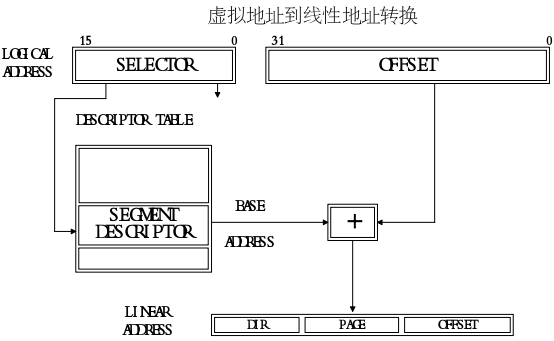
\includegraphics{figures/3.15.1.png}
\caption{3.15.1}
\end{figure}

图1 分段机制中虚拟地址到线性地址转换转换基本过程

分段存储管理机制需要在启动保护模式的前提下建立。从上图可以看出,为了使得分段存储管理机制正常运行,需要在启动保护模式前建立好段描述符和段描述符表(参看bootasm.S中的``lgdt
gdtdesc''语句和gdt标号/gdtdesc标号下的数据结构)。

\subsubsection{段选择子}\label{ux6bb5ux9009ux62e9ux5b50}

\textbf{段选择子}是用来选择哪个描述符表和在该表中索引哪一个描述符的。选择子可以做为指针变量的一部分,从而对应用程序员是可见的,但是一般是由编译器(gcc)和链接工具(ld)来设置的。段选择子的内容一般放在段寄存器中。选择子的格式如下图所示:

\begin{figure}[htbp]
\centering
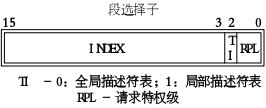
\includegraphics{figures/3.15.2.png}
\caption{3.15.2}
\end{figure}

图2 段选择子结构

\textbf{索引(Index)}:在描述符表中从8192个描述符中选择一个描述符。处理器自动将这个索引值乘以8(描述符的长度),再加上描述符表的基址来索引描述符表,从而选出一个合适的描述符。

\textbf{表指示位(Table
Indicator,TI)}:选择应该访问哪一个描述符表。0代表应该访问全局描述符表(GDT);1代表应该访问局部描述符表(LDT)。LDT在实验中没有涉及。

\textbf{请求特权级(Requested Privilege
Level,RPL)}:用于段级的保护机制,比如,段选择子是CS,则这两位表示当前执行指令的处理器所处的特权级的值,从而你可以了解到当前处理器是处于用户态(Ring
3)还是内核态(Ring 0)。在后续试验中会进一步讲解。

\subsubsection{段描述符}\label{ux6bb5ux63cfux8ff0ux7b26}

在分段存储管理机制的保护模式下,每个段由如下三个参数进行定义:段基地址(Base
Address)、段界限(Limit)和段属性(Attributes)。

\textbf{段基地址}:即线性地址空间中段的起始地址。在80386保护模式下,段基地址长32位。因为基地址长度与寻址地址的长度相同,所以任何一个段都可以从32位线性地址空间中的任何一个字节开始,而不象实方式下规定的边界必须被16整除。
在实验中,一般都简化了段机制的使用,把所有段的段基地址设置为0。

\textbf{段界限}:规定段的大小。在80386保护模式下,段界限用20位表示,而且段界限可以是以单字节为最小单位或以4K字节为最小单位。在实验中,一般都简化了段机制的使用,把所有段的段界限设置为0xFFFFF,以4K字节为最小单位,即段的界限为4GB;

\textbf{类型(TYPE)}:用于区别不同类型的描述符。可表示所描述的段是代码段还是数据段,所描述的段是否可读/写/执行,段的扩展方向等。
\textbf{描述符特权级(Descriptor Privilege
Level)(DPL)}:用来实现保护机制。 \textbf{段存在位(Segment-Present
bit)}:如果这一位为0,则此描述符为非法的,不能被用来实现地址转换。如果一个非法描述符被加载进一个段寄存器,处理器会立即产生异常。图2显示了当存在位为0时,描述符的格式。操作系统可以任意的使用被标识为可用(AVAILABLE)的位。
\textbf{已访问位(Accessed
bit)}:当处理器访问该段(当一个指向该段描述符的选择子被加载进一个段寄存器)时,将自动设置访问位。操作系统可清除该位。
上述表示段的属性的参数通过段描述符(Segment
Descriptor)来表示,一个段描述符占8字节。段描述符的结构如下图所示:

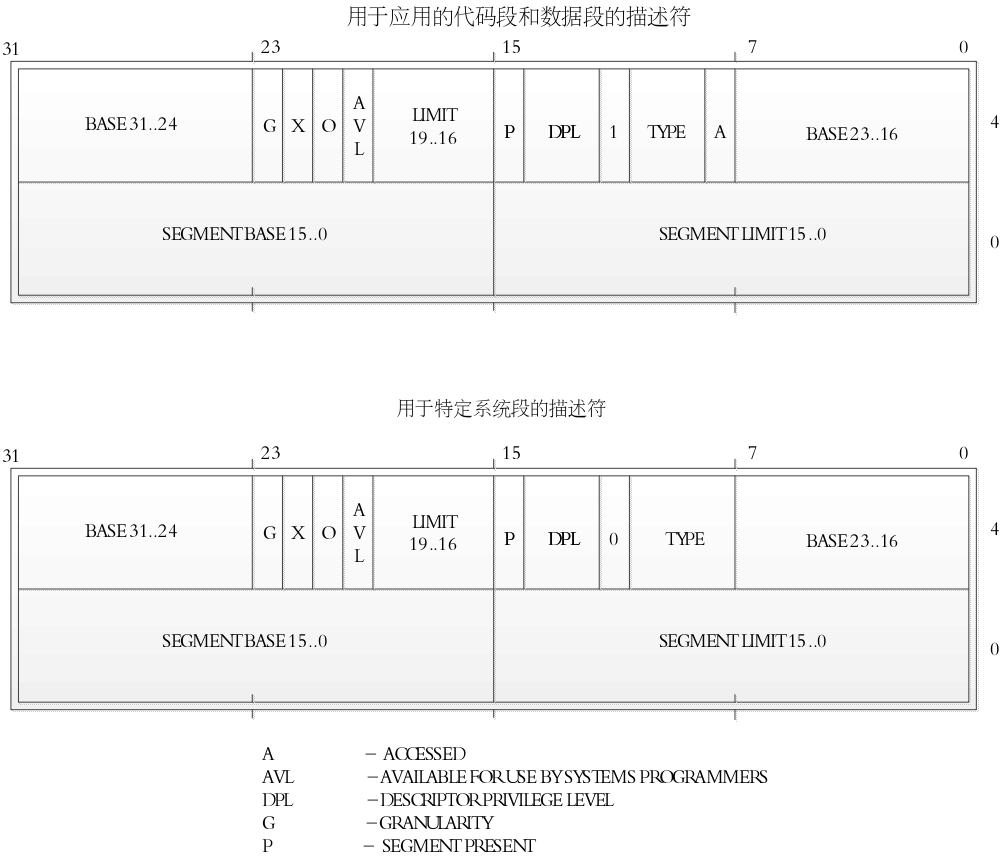
\includegraphics{figures/3.15.3.png} 图2 段描述符结构

\subsubsection{全局描述符表}\label{ux5168ux5c40ux63cfux8ff0ux7b26ux8868}

全局描述符表的是一个保存多个段描述符的``数组'',其起始地址保存在全局描述符表寄存器GDTR中。GDTR长48位,其中高32位为基地址,低16位为段界限。由于GDT
不能用GDT本身之内的描述符进行描述定义,所以采用GDTR寄存器来表示GDT这一特殊的系统段。注意,全部描述符表中第一个段描述符设定为空段描述符。GDTR中的段界限以字节为单位。对于含有N个描述符的描述符表的段描述符实际所占空间通常可设为8\emph{N,若起始地址为gdt\_base,则结束地址为gdt\_base+8}N-1。可参考proj1中的bootasm.S中的gdt标号和gdtdesc标号下的内容,以及lgdt指令的操作数。
全局描述符表的第一项是不能被CPU使用,所以当一个段选择子的索引(Index)部分和表指示位(Table
Indicator)都为0的时(即段选择子指向全局描述符表的第一项时),可以当做一个空的选择子。当一个段寄存器被加载一个空选择子时,处理器并不会产生一个异常。但是,当用一个空选择子去访问内存时,则会产生异常。在proj1的实验中,值设置了三个段描述符,即NULL段、TEXT段和DATA段(都是4GB的访问范围)。

\subsection{分段机制的系统寄存器}\label{ux5206ux6bb5ux673aux5236ux7684ux7cfbux7edfux5bc4ux5b58ux5668}

80386
有4个寄存器来寻址描述发表等系统数据结构,用来实现段式内存管理。内存管理寄存器包括:

\begin{itemize}
\tightlist
\item
  全局描述符表寄存器 (Global Descriptor Table Register,GDTR
  ):指向全局段描述符表 GDT
\item
  局部描述符表寄存器 (Local Descriptor Table
  Register,LDTR):指向局部段描述符表 LDT~(目前用不上)
\item
  中断门描述符表寄存器 (Interrupt Descriptor Table
  Register,IDTR):指向一张包含中断处理子程序入口点的表(IDT)~
\item
  任务寄存器 (Task
  Register,TR):这个寄存器指向当前任务信息存放处,这些信息是处理器进行任务切换所需要的。(目前用不上)
  80386有四个32位的控制寄存器,分别命名位CR0、CR1、CR2和CR3。CR0包含指示处理器工作方式、启用和禁止分页管理机制、控制浮点协处理器操作的控制位。具体描述如下:
\item
  PE(保护模式允许 Protection Enable,比特位 0):设置PE
  将让处理器工作在保护模式下。复位PE将返回到实模式工作。
\item
  PG(分页允许 Paging, 比特位 31): PG
  指明处理器是否通过页表来转换线性地址到物理地址。在后续试验中将讲述如何设置PG位。
  CR0中的位5\textasciitilde{}位30是保留位,这些位的值必须为0。CR2及CR3由分页管理机制使用,将在后续试验中讲述。在80386中不能使用CR1,否则会引起无效指令操作异常。
\end{itemize}

\section{【实现】实模式到保护模式的切换}\label{ux5b9eux73b0ux5b9eux6a21ux5f0fux5230ux4fddux62a4ux6a21ux5f0fux7684ux5207ux6362}

BIOS把bootloader从硬盘(即是我们刚才生成的ucore.img)的第一个扇区(即是我们刚才生成的bootblock)读出来并拷贝到内存一个特定的地址0x7c00处,然后BIOS会跳转到那个地址((即CS=0,EIP=0x7c00))继续执行。至此BIOS的初始化工作做完了,进一步的工作交给了ucore的bootloader。

bootloader从哪里开始执行呢?我们【实验2-2
编译运行bootloader】中描述make工作过程的第五步就是生成了一个bootblock.asm,它的前面几行是:

\begin{lstlisting}
    obj/bootblock.o:     file format elf32-i386
    Disassembly of section .text:
    00007c00 <start>:
    .set CR0_PE_ON,      0x1         # protected mode enable flag
    .globl start
    start:
      .code16                     # Assemble for 16-bit mode
      cli                         # Disable interrupts
      7c00: fa                    cli
\end{lstlisting}

上述代码片段指出了bootblock(即bootloader)在0x7c00虚拟地址(在这里虚拟地址=线性地址=物理地址)处的指令为``cli'',如果读者再回头看看bootasm.S中的12\textasciitilde{}15行:

\begin{lstlisting}
    .globl start
    start:
      .code16                     # Assemble for 16-bit mode
      cli                         # Disable interrupts
      cld                         # String operations increment
\end{lstlisting}

就可以发现二者是完全一致的。而这个虚拟地址的设定是通过链接器ld完成的,我们【实验2-2
编译运行bootloader】中描述make工作过程的第四步: i386-elf-ld -N -e start
-Ttext 0x7C00 -o obj/bootblock.o obj/bootasm.o obj/bootmain.o

其中``-e start''指出了bootblock的入口地址为start,而``-Ttext
0x7C00''指出了代码段的起始地址为0x7c00,这也就导致start位置的虚拟地址为0x7c00。

从0x7c00开始,bootloader用了21条汇编指令完成了初始化和切换到保护模式的工作。其具体步骤如下:

\begin{enumerate}
\def\labelenumi{\arabic{enumi}.}
\item
  关中断,并清除方向标志,即将DF置``0'',这样(E)SI及(E)DI的修改为增量。
  cli \# Disable interrupts cld \# String operations increment
\item
  清零各数据段寄存器:DS、ES、FS xorw \%ax,\%ax \# Segment number zero
  movw \%ax,\%ds \# -\textgreater{} Data Segment movw \%ax,\%es \#
  -\textgreater{} Extra Segment movw \%ax,\%ss \# -\textgreater{} Stack
  Segment
\item
  使能A20地址线,这样80386就可以突破1MB访存现在,而可访问4GB的32位地址空间了。可回顾2.2.1节的【历史:A20地址线与处理器向下兼容】。
  seta20.1: inb \$0x64,\%al \# Wait for not busy testb \$0x2,\%al jnz
  seta20.1 movb \$0xd1,\%al \# 0xd1 -\textgreater{} port 0x64 outb
  \%al,\$0x64 seta20.2: inb \$0x64,\%al \# Wait for not busy testb
  \$0x2,\%al jnz seta20.2 movb \$0xdf,\%al \# 0xdf -\textgreater{} port
  0x60 outb \%al,\$0x60
\item
  建立全局描述符表(可回顾2.2.3节对全局描述符表的介绍),使能80386的保护模式(可回顾2.2.4节对CR0寄存器的介绍)。lgdt指令把gdt表的起始地址和界限(gdt的大小-1)装入GDTR寄存器中。而指令``movl
  \%eax,\%cr0''把保护模式开启位置为1,这时已经做好进入80386保护模式的准备,但还没有进入80386保护模式
  lgdt gdtdesc movl \%cr0, \%eax orl \$CR0\_PE\_ON, \%eax movl \%eax,
  \%cr0

  gdtdesc指出了全局描述符表(可以看成是段描述符组成的一个数组)的起始位置在gdt符号处,而gdt符号处放置了三个段描述符的信息
  gdt: SEG\_NULLASM \# null seg SEG\_ASM(STA\_X\textbar{}STA\_R, 0x0,
  0xffffffff) \# code seg SEG\_ASM(STA\_W, 0x0, 0xffffffff) \# data seg
  每个段描述符占8个字节,第一个是NULL段描述符,没有意义,表示全局描述符表的开始,紧接着是代码段描述符(位于全局描述符表的0x8处的位置),具有可读(STA\_R)和可执行(STA\_X)的属性,并且段起始地址为0,段大小为4GB;接下来是数据段描述符(位于全局描述符表的0x10处的位置),具有可读(STA\_R)和可写(STA\_W)的属性,并且段起始地址为0,段大小为4GB。
\item
  通过长跳转指令进入保护模式。80386在执行长跳转指令时,会重新加载\(PROT_MODE_CSEG的值(即0x8)到CS中,同时把\)protcseg的值赋给EIP,这样80386就会把CS的值作为全局描述符表的索引来找到对应的代码段描述符,设定当前的EIP为0x7c32(即protcseg标号所在的段内偏移),
  根据2.2.3节描述的分段机制中虚拟地址到线性地址转换转换的基本过程,可以知道线性地址(即物理地址)为:
  gdt{[}CS{]}.base\_addr+EIP=0x0+0x7c32=0x7c32 ljmp \$PROT\_MODE\_CSEG,
  \$protcseg
\item
  执行完上面的这条汇编语句后,bootloader让80386从实模式进入了保护模式。由于在访问数据或栈时需要用DS/ES/FS/GS和SS段寄存器作为全局描述符表的下标来找到相应的段描述符,所以还需要对DS/ES/FS/GS和SS段寄存器进行初始化,使它们都指向位于0x10处的段描述符(即gdt中的数据段描述符)。
  movw \$PROT\_MODE\_DSEG, \%ax \# Our data segment selector movw \%ax,
  \%ds \# -\textgreater{} DS: Data Segment movw \%ax, \%es \#
  -\textgreater{} ES: Extra Segment movw \%ax, \%fs \# -\textgreater{}
  FS movw \%ax, \%gs \# -\textgreater{} GS movw \%ax, \%ss \#
  -\textgreater{} SS: Stack Segment

  在保护模式下,所有的内存寻址将经过分段机制的存储管理来完成,即每个虚拟地址访问将经过分段机制转换成线性地址,由于这时还没有启动分页模式,所以线性地址就是物理地址。
\end{enumerate}

\section{【实现】设置栈}\label{ux5b9eux73b0ux8bbeux7f6eux6808}

只有设置好的合适大小和地址的栈内存空间(简称栈空间),才能有效地进行函数调用。这里为了减少汇编代码量,我们就通过C代码来完成显示。由于需要调用C语言的函数,所以需要自己建立好栈空间。设置栈的代码如下:

\begin{lstlisting}
movl    $start, %esp
\end{lstlisting}

由于start位置(0x7c00)前的地址空间没有用到,所以可以用来作为bootloader的栈,需要注意栈是向下长的,所以不会破坏start位置后面的代码。在后面的小节还会对栈进行更加深入的讲解。我们可以通过用gdb调试bootloader来进一步观察栈的变化:

\textbf{【实验】用gdb调试bootloader观察栈信息 }

\begin{enumerate}
\def\labelenumi{\arabic{enumi}.}
\item
  开两个窗口;在一个窗口中,在proj1目录下执行命令make;
\item
  在proj1目录下执行 ``qemu -hda bin/ucore.img -S
  -s'',这时会启动一个qemu窗口界面,处于暂停状态,等待gdb链接;
\item
  在另外一个窗口中,在proj1目录下执行命令 gdb obj/bootblock.o;
\item
  在gdb的提示符下执行如下命令,会有一定的输出:

\begin{lstlisting}
    (gdb) target remote :1234   #与qemu建立远程链接
    (gdb) break bootasm.S:68    #在bootasm.S的第68行“movl $start, %esp”设置一个断点
    (gdb) continue              #让qemu继续执行  
\end{lstlisting}

  这时qemu会继续执行,但执行到bootasm.S的第68行时会暂停,等待gdb的控制。这时可以在gdb中继续输入如下命令来分析栈的变化:

\begin{lstlisting}
    (gdb) info registers esp
    esp            0xffd6   0xffd6    #没有执行第68行代码前的esp值
    (gdb) si                          #执行第68行代码
    69        call bootmain
    (gdb) info registers esp
    esp            0x7c00   0x7c00   #当前的esp值,即栈顶
    (gdb) si
    bootmain () at boot/bootmain.c:87    #执行call汇编指令
    87      bootmain(void) {
    (gdb) info registers esp
    esp            0x7bfc   0x7bfc    #当前的esp值0x7bfc, 0x7bfc处存放了bootmain函数的返回地址0x7c4a,这可以通过下面两个命令了解  
    (gdb) x /4x 0x7bfc                  
    0x7bfc: 0x00007c4a      0xc031fcfa      0xc08ed88e      0x64e4d08e
    (gdb) x /4i 0x7c40
       0x7c40 <protcseg+14>:        mov    $0x7c00,%esp
       0x7c45 <protcseg+19>:        call   0x7c6c <bootmain>
       0x7c4a <spin>:       jmp    0x7c4a <spin>
       0x7c4c <gdt>:        add    %al,(%eax)
\end{lstlisting}
\end{enumerate}

\subsection{【提示】}\label{ux63d0ux793a}

在proj1中执行

\begin{lstlisting}
    make debug
\end{lstlisting}

则自动完成上述大部分前期工作,即qemu和gdb的加载,且gdb会自动建立于qemu的联接并设置好断点。具体实现可参看proj1的Makefile中于debug相关的内容和tools/gdbinit中的内容。

\section{【实现】显示字符串}\label{ux5b9eux73b0ux663eux793aux5b57ux7b26ux4e32}

bootloader只在CPU和内存中打转无法让读者很容易知道bootloader的工作是否正常,为此在成功完成了保护模式的转换后,就需要通过显示字符串来展示一下自己了。bootloader设置好栈后,就可以调用bootmain函数显示字符串了。在proj1中使用了显示器和并口两种外设来显示字符串,主要的代码集中在bootmain.c中。

这里采用的是很简单的基于Programmed I/O
(PIO)方式,PIO方式是一种通过CPU执行I/O端口指令来进行数据读写的数据交换模式,被广泛应用于硬盘、光驱等设备的基础传输模式中。这种I/O访问方式使用CPU
I/O端口指令来传送所有的命令、状态和数据,需要CPU全程参与,效率较低,但编程很简单。后面讲到的中断方式将更加高效。
在bootmain.c中的lpt\_putc函数完成了并口输出字符的工作。输出一个字符的流程(可参看bootmain.c中的lpc\_putc函数实现)大致如下:

\begin{enumerate}
\def\labelenumi{\arabic{enumi}.}
\tightlist
\item
  读I/O端口地址0x379,等待并口准备好;
\item
  向I/O端口地址0x378发出要输出的字符;
\item
  向I/O端口地址0x37A发出控制命令,让并口处理要输出的字符。
\end{enumerate}

在bootmain.c中的serial\_putc函数完成了串口输出字符的工作。输出一个字符的流程(可参看bootmain.c中的serial\_putc函数实现)大致如下:

\begin{enumerate}
\def\labelenumi{\arabic{enumi}.}
\tightlist
\item
  读I/O端口地址(0x3f8+5)获得LSR寄存器的值,等待串口输出准备好;
\item
  向I/O端口地址0x3f8发出要输出的字符;
\end{enumerate}

在bootmain.c中的cga\_putc函数完成了CGA字符方式在某位置输出字符的工作。输出一个字符的流程(可参看bootmain.c中的cga\_putc函数实现)大致如下:

\begin{enumerate}
\def\labelenumi{\arabic{enumi}.}
\tightlist
\item
  写I/O端口地址0x3d4,读I/O端口地址0x3d5,获得当前光标位置;
\item
  在光标的下一位置的显存地址空间上写字符,格式是黑色背景/白色字符;
\item
  设置当前光标位置为下一位置。
\end{enumerate}

proj1启动后的PC机内存布局如下图所示:

\begin{figure}[htbp]
\centering
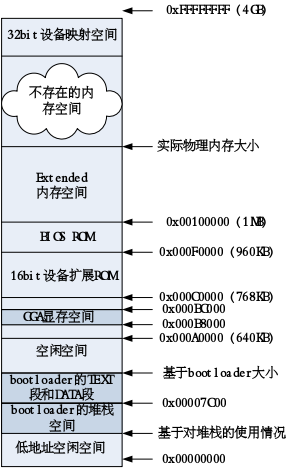
\includegraphics{figures/3.18.1.png}
\caption{3.18.1}
\end{figure}

自此,我们了解了一个小巧的bootloader的实现过程,但这还仅仅是百尺竿头的第一步,它还只能显示字符串,不能加载操作系统。我们还需要扩展bootloader的功能,让它能够加载操作系统。


\section{可读ELF格式文件的baby
bootloader}\label{ux53efux8bfbelfux683cux5f0fux6587ux4ef6ux7684baby-bootloader}

\subsection{实验目标}\label{ux5b9eux9a8cux76eeux6807}

接下来,我们需要完成一个能够读取位于硬盘中OS的代码内容并加载运行OS的bootloader,这需要bootloader能够读取硬盘扇区中的数据。由于OS采用ELF执行文件格式,所以bootloader能够解析ELF格式文件,把其中的代码和数据放到内存中正确的位置。Bootloader虽然增加了这么多功能,但整个bootloader的大小还是必须小于512个字节,这样才能放到只有512字节大小的硬盘主引导扇区中。
\textgreater{}
ucore内核不一定非要是ELF格式,基于binary格式的ucore内核也可以被bootloader识别与加载。

通过分析和实现这个bootloader,读者对设备管理的方式会有更加深入的理解,掌握bootloader/操作系统等底层系统软件是如何在保护模式下通过PIO(Programming
I/O,可编程I/O)方式访问块设备硬盘;理解如何在保护模式下解析并加载一个简单的ELF执行文件。

\subsection{proj2/3概述}\label{proj23ux6982ux8ff0}

\subsubsection{实现描述}\label{ux5b9eux73b0ux63cfux8ff0}

proj2基于proj1的主要实现一个可读硬盘并可分析ELF执行文件格式的bootloader,由于bootloader要放在512字节大小的主引导扇区中,所以不得不去掉部分显示输出的功能,确保整个bootloader的大小小于510个字节(最后两个字节用于硬盘主引导扇区标识,即``55AA'')。proj3在proj2的基础上增加了一个只能显示字符的第一代幼稚型操作系统ucore,用来验证proj2实现的bootloader能够正确从硬盘读出ucore并加载到正确的内存位置,并能把CPU控制权交给ucore。ucore在获得CPU控制权后,能够在保护模式下显示一个字符串,表明自己能够正常工作了

\subsubsection{项目组成}\label{ux9879ux76eeux7ec4ux6210}

这里我们分了两个project来完成此事。proj2是一个可分析ELF执行文件格式的例子,proj2整体目录结构如下所示:

\begin{lstlisting}
        proj2/
        |-- boot
        |   |-- asm.h
        |   |-- bootasm.S
        |   `-- bootmain.c
        |-- libs
        |   |-- elf.h
        |   |-- types.h
        |   `-- x86.h
        |-- Makefile
        ……
\end{lstlisting}

proj2与proj1类似,只是增加了libs/elf.h文件,并且bootmain.c中增加了对ELF执行文件的简单解析功能和读磁盘功能。

proj3建立在proj2基础之上,增加了一个只能显示字符的ucore操作系统,让bootloader能够把这个操作系统从硬盘上读到内存中,并跳转到ucore的起始处执行ucore的功能。proj3整体目录结构如下所示:

\begin{lstlisting}
        proj3
        |-- boot
        |   |-- asm.h
        |   |-- bootasm.S
        |   `-- bootmain.c
        |-- kern
        |   |-- driver
        |   |   |-- console.c
        |   |   `-- console.h
        |   |-- init
        |   |   `-- init.c
        |   `-- libs
        |       `-- stdio.c
        |-- libs
        |   |-- elf.h
        |   |-- error.h
        |   |-- printfmt.c
        |   |-- stdarg.h
        |   |-- stdio.h
        |   |-- string.c
        |   |-- string.h
        |   |-- types.h
        |   `-- x86.h
        |-- Makefile
        ……
\end{lstlisting}

proj3相对于proj2增加了ucore相关的文件,下面简要说明一下: *
libs目录下的printfmt.c:完成类似C语言的printf中的格式化处理; *
libs目录下的string.c:完成类似C语言的str***相关的字符串处理函数; *
libs目录下的st\emph{.h:是支持上述两个库函数(可被内核和用户应用共享)的.h文件;
} kern/init目录下的init.c:完成ucore的初始化工作; *
kern/driver目录下的console.c:提供并口/串口/CGA方式的字符输出的console驱动;
* kern/libs/stdio.c:提供内核方式下的的cprintf函数功能;

\subsubsection{编译运行}\label{ux7f16ux8bd1ux8fd0ux884c}

那接下来是如何生成一个包含了bootloader和ucore操作系统的硬盘镜像呢?我们先修改proj3目录下的Makefile,在其第五行

\begin{lstlisting}
        V       := @
\end{lstlisting}

的最前面增加一个``\#''(目的是让make工具程序详细显示整个project的编译过程),这样就把这行给注释了。然后在proj3目录下执行make,可以看到:

\begin{lstlisting}
        ……
        ld -m    elf_i386 -Ttext 0x100000 -e kern_init -o bin/kernel obj/kern/init/init.o obj/kern/libs/printf.o obj/kern/driver/console.o obj/libs/printfmt.o obj/libs/string.o
        ……
        dd if=bin/kernel of=bin/ucore.img seek=1 conv=notrunc
\end{lstlisting}

这两步是生成ucore的关键。第一步把ucore涉及的各个.o目标文件链接起来,并在bin目录下形成ELF文件格式的文件kernel,这就是我们第一个ucore操作系统,而且设定ucore的执行入口地址在0x10000,即kern\_init函数的起始位置。这也就意味着bootloader需要把读出的kernel文件的代码段+数据段放置在0x10000起始的内存空间。第二步是把bin目录下的kernel文件直接覆盖到ucore.img(虚拟硬盘的文件)的bootloader所处扇区(即第一个扇区,主引导扇区)之后的扇区(第二个扇区)。如果一个扇区大小为512字节,这kernel覆盖的扇区数为上取整(kernel的大小/512字节)。

编译后运行proj3的示意图如下所示:

%\begin{lstlisting}
%![qemu_cha1](figures/qemu_cha2.jpg)
%\end{lstlisting}


\section{【背景】访问硬盘数据控制}\label{ux80ccux666fux8bbfux95eeux786cux76d8ux6570ux636eux63a7ux5236}

bootloader让80386处理器进入保护模式后,下一步的工作就是从硬盘上加载并运行OS。考虑到实现的简单性,bootloader的访问硬盘都是LBA模式的PIO(Program
IO)方式,即所有的I/O操作是通过CPU访问硬盘的I/O地址寄存器完成。

一般主板有2个IDE通道(是硬盘的I/O控制器),每个通道可以接2个IDE硬盘。第一个IDE通道通过访问I/O地址0x1f0-0x1f7来实现,第二个IDE通道通过访问0x170-0x17f实现。每个通道的主从盘的选择通过第6个I/O偏移地址寄存器来设置。具体参数见下表。

\begin{lstlisting}
I/O地址   功能
0x1f0   读数据,当0x1f7不为忙状态时,可以读。
0x1f2   要读写的扇区数,每次读写前,需要指出要读写几个扇区。
0x1f3   如果是LBA模式,就是LBA参数的0-7位
0x1f4   如果是LBA模式,就是LBA参数的8-15位
0x1f5   如果是LBA模式,就是LBA参数的16-23位
0x1f6   第0~3位:如果是LBA模式就是24-27位   第4位:为0主盘;为1从盘
第6位:为1=LBA模式;0 = CHS模式     第7位和第5位必须为1
0x1f7   状态和命令寄存器。操作时先给命令,再读取内容;如果不是忙状态就从0x1f0端口读数据
\end{lstlisting}

硬盘数据是储存到硬盘扇区中,一个扇区大小为512字节。读一个扇区的流程大致为通过outb指令访问I/O地址:0x1f2\textasciitilde{}-0x1f7来发出读扇区命令,通过in指令了解硬盘是否空闲且就绪,如果空闲且就绪,则通过inb指令读取硬盘扇区数据都内存中。可进一步参看bootmain.c中的readsect函数实现来了解通过PIO方式访问硬盘扇区的过程。

\section{【背景】理解ELF文件格式}\label{ux80ccux666fux7406ux89e3elfux6587ux4ef6ux683cux5f0f}

由于本章的project中,bootloader会访问ELF(Executable and linking
format)格式的ucore,并把ucore加载到内存中。所以,在这里我们需要简单介绍一下ELF文件格式,以帮助我们理解ucore的整个编译、链接和加载的过程,特别是希望读者对ld链接器用到的链接地址(Link
address)和操作系统相关的加载地址(Load address)有更清楚的了解。

ELF文件格式是Linux系统下的一种常用目标文件(object
file)格式,有三种主要类型。可重定位文件(relocatable
file)类型和共享目标文件(shared object
file)类型在本实验中没有涉及。本实验的OS文件类型是可执行文件(executable
file)类型,这种ELF文件格式类型提供程序的进程映像,加载程序的内存地址描述等。

简单地说,bootloader通过解析ELF格式的ucore,可以了解到ucore的代码段(机器码)/数据段(初始化的变量)等在文件中的位置和大小,以及应该放到内存中的位置;可了解ucore的BSS段(未初始化的变量,具体内容没有保存在文件中)的内存位置和大小。这样bootloader就可以把ucore正确地放置到内存中,便于ucore的正确执行。

这里只分析与本章相关的ELF可执行文件类型。ELF的执行文件映像如下所示:

\begin{figure}[htbp]
\centering
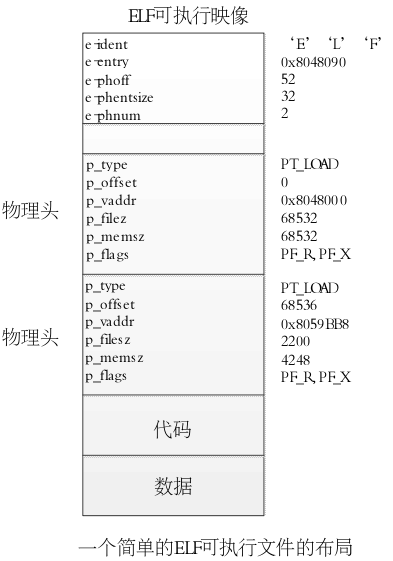
\includegraphics{figures/3.2.4.1.png}
\caption{3.2.4.1}
\end{figure}

ELF的文件头包含整个执行文件的数据结构elf
header,描述了整个执行文件的组织结构。其定义在proj2/3中的elf.h文件中:

\begin{lstlisting}
struct elfhdr {
    uint32_t e_magic;     // must equal ELF_MAGIC
    uint8_t e_elf[12];
    uint16_t e_type;      // 1=relocatable, 2=executable, 3=shared object, 4=core image
    uint16_t e_machine;   // 3=x86, 4=68K, etc.
    uint32_t e_version;   // file version, always 1
    uint32_t e_entry;     // entry point if executable
    uint32_t e_phoff;     // file position of program header or 0
    uint32_t e_shoff;     // file position of section header or 0
    uint32_t e_flags;     // architecture-specific flags, usually 0
    uint16_t e_ehsize;    // size of this elf header
    uint16_t e_phentsize; // size of an entry in program header
    uint16_t e_phnum;     // number of entries in program header or 0
    uint16_t e_shentsize; // size of an entry in section header
    uint16_t e_shnum;     // number of entries in section header or 0
    uint16_t e_shstrndx;  // section number that contains section name strings
};
\end{lstlisting}

program
header描述与程序执行直接相关的目标文件结构信息,用来在文件中定位各个段的映像,同时包含其他一些用来为程序创建进程映像所必需的信息。可执行文件的程序前面部分有一个program
header结构的数组,
每个结构描述了一个``段''(segment)或者准备程序执行所必需的其它信息。目标文件的
``段''(segment) 包含一个或者多个 ``节区''(section)
,也就是``段内容(Segment Contents)'' 。program
header仅对于可执行文件和共享目标文件有意义。可执行目标文件在elfhdr的e\_phentsize和e\_phnum成员中给出其自身程序头部的大小。程序头部的数据结构如下表所示:

\begin{lstlisting}
struct proghdr {
    uint32_t p_type;   // loadable code or data, dynamic linking info,etc.
    uint32_t p_offset; // file offset of segment
    uint32_t p_va;     // virtual address to map segment
    uint32_t p_pa;     // physical address, not used
    uint32_t p_filesz; // size of segment in file
    uint32_t p_memsz;  // size of segment in memory (bigger if contains bss)
    uint32_t p_flags;  // read/write/execute bits
    uint32_t p_align;  // required alignment, invariably hardware page size
};
\end{lstlisting}

\textbf{链接地址(Link address)和加载地址(Load address)}

Link~Address是指编译器指定代码和数据所需要放置的内存地址,由链接器配置。Load~Address是指程序被实际加载到内存的位置。一般由可执行文件结构信息和加载器可保证这两个地址相同。Link
Addr和LoadAddr不同会导致:

\begin{lstlisting}
直接跳转位置错误
直接内存访问(只读数据区或bss等直接地址访问)错误
堆和栈等的使用不受影响,但是可能会覆盖程序、数据区域
\end{lstlisting}

也存在Link地址和Load地址不一样的情况(如动态链接库)。在proj3中,bootloader和ucore的链接地址和加载地址是一致的。

\begin{figure}[htbp]
\centering
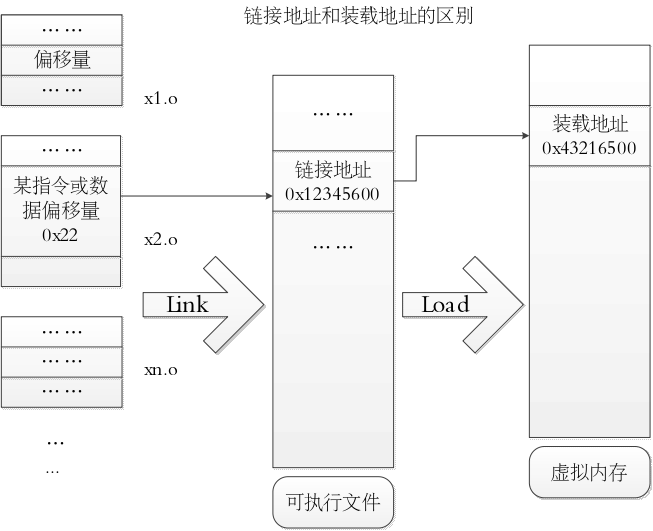
\includegraphics{figures/3.2.4.2.png}
\caption{3.2.4.2}
\end{figure}

\section{【背景】操作系统执行代码的组成}\label{ux80ccux666fux64cdux4f5cux7cfbux7edfux6267ux884cux4ee3ux7801ux7684ux7ec4ux6210}

ucore通过gcc编译和ld链接,形成了ELF格式执行文件kernel(位于bin目录下),这样kernel的内部组成与一般的应用程序差别不大。一般而言,一个执行程序的内容是至少由
bss段、data段、text段三大部分组成。 * BSS段:BSS(Block Started by
Symbol)段通常是指用来存放执行程序中未初始化的全局变量的一块存储区域。BSS段属于静态内存分配的存储空间。
* 数据段:数据段(Data
Segment)通常是指用来存放执行程序中已初始化的全局变量的一块存储区域。数据段属于静态内存分配的存储空间。
* 代码段:代码段(Code Segment/Text
Segment)通常是指用来存放程序执行代码的一块存储区域。这部分区域的大小在程序运行前就已经确定,并且内存区域通常属于只读,
某些CPU架构也允许代码段为可写,即允许修改程序。在代码段中,也有可能包含一些只读的常数变量,例如字符串常量等。

ucore和一般应用程序一样,首先是保存在像硬盘这样的非易失性存储介质上,当需要运行时,被加载到内存中。这时,需要把代码段、数据段的内容拷贝到内存中。对于位于BSS段中的未初始化的全局变量,执行程序一般认为其值为零。所以需要把BSS段对应的内存空间清零,确保执行代码的正确运行。可查看init文件中的kern\_init函数的第一个执行语句``memset(edata,
0, end - edata);''。

随着ucore的执行,可能需要进行函数调用,这就需要用到栈(stack);如果需要动态申请内存,这就需要用到堆(heap)。堆和栈是在操作系统执行过程中动态产生和变化的,并不存在于表示内核的执行文件中。栈又称堆栈,
是用户存放程序临时创建的局部变量,即函数中定义的变量(但不包括static声明的变量,static意味着在数据段中存放变量)。除此以外,在函数被调用时,其参数也会被压入发起调用函数的栈中,并且待到调用结束后,函数的返回值也会被存放回栈中。由于栈的先进后出特点,所以栈特别方便用来保存/恢复调用现场。可以把栈看成一个寄存、交换临时数据的内存区。堆是用于存放运行中被动态分配的内存空间,它的大小并不固定,可动态扩张或缩减,这需要操作系统自己进行有效的管理。

\section{【实现】bootloader加载并运行ucore}\label{ux5b9eux73b0bootloaderux52a0ux8f7dux5e76ux8fd0ux884cucore}

了解完proj2/3的组成与编译,并大致理解上述两个背景知识后,我们就可以分析bootloader加载并运行ucore操作系统的工作流程。

硬盘数据是储存到硬盘扇区中,一个扇区大小为512字节。读一个扇区的流程可参看bootmain.c中的readsect函数实现。大致如下:

\begin{enumerate}
\def\labelenumi{\arabic{enumi}.}
\tightlist
\item
  读I/O地址0x1f7,等待磁盘准备好;
\item
  写I/O地址0x1f2\textasciitilde{}0x1f5,0x1f7,发出读取第offseet个扇区处的磁盘数据的命令;
\item
  读I/O地址0x1f7,等待磁盘准备好;
\item
  连续读I/O地址0x1f0,把磁盘扇区数据读到指定内存。
\end{enumerate}

这个函数是被bootloader用于读取硬盘上的ucore操作系统。bootloader为了读取硬盘上的ucore操作系统,将调用bootmain函数首先读取了位于主引导扇区的后的连续8个扇区(可参见bootmain函数中的第一条语句),并把数据放到0x10000处(可回顾一下2.7.1中描述链接bin/kernel的过程),并按照数据结构elfhdr来解析这块4KB大小的数据;如果其e\_magic数据域不等于ELF\_MAGIC(即0x464C457F),则表示这个不是标准的ELF格式的文件;如果等于ELF\_MAGIC,则继续解析,并根据其e\_phnum数据域的值来读取多个program
header,并根据program
header的信息,了解到ucore中各个segment的起始位置和大小,然后把放在硬盘上的相关segment读入到内存中。

\textbf{【实验】分析kernel并在bootloader中显示kernel的segment信息}

\begin{enumerate}
\def\labelenumi{\arabic{enumi}.}
\item
  在proj3目录下执行命令make,则会在bin目录下生成kernel,即ELF执行格式文件的操作系统ucore;
\item
  在proj3目录下执行命令 readelf -h bin/kernel,可得到有关elf
  header的如下信息

\begin{lstlisting}
ELF Header:
  Magic:   7f 45 4c 46 01 01 01 00 00 00 00 00 00 00 00 00 
  Class:                             ELF32
  Data:                              2's complement, little endian
  Version:                           1 (current)
  OS/ABI:                            UNIX - System V
  ABI Version:                       0
  Type:                              EXEC (Executable file)
  Machine:                           Intel 80386
  Version:                           0x1
  Entry point address:               0x100000
  Start of program headers:          52 (bytes into file)
  Start of section headers:          19872 (bytes into file)
  Flags:                             0x0
  Size of this header:               52 (bytes)
  Size of program headers:           32 (bytes)
  Number of program headers:         3
  Size of section headers:           40 (bytes)
  Number of section headers:         17
  Section header string table index: 14
\end{lstlisting}

  从中,我们可以看到kernel的入口点在0x100000,program
  header相对文件的偏移位置在52,elf header的大小为52字节,program
  header的大小为32字节。
\item
  在proj3目录下执行命令 readelf -l bin/kernel,可得到有关program
  header的如下信息 Elf file type is EXEC (Executable file) Entry point
  0x100000 There are 3 program headers, starting at offset 52

\begin{lstlisting}
Program Headers:
  Type           Offset   VirtAddr   PhysAddr   FileSiz MemSiz  Flg Align
  LOAD           0x001000 0x00100000 0x00100000 0x01038 0x01038 R E 0x1000
  LOAD           0x002038 0x00102038 0x00102038 0x00004 0x00004 RW  0x1000
  GNU_STACK      0x000000 0x00000000 0x00000000 0x00000 0x00000 RW  0x4

 Section to Segment mapping:
  Segment Sections...
   00     .text .rodata 
   01     .data 
   02     
\end{lstlisting}
\end{enumerate}

从中,我们可以看到kernel的入口点在0x100000,代码段位于0x100000,大小为0x1038;数据段位于0x102038,大小为0x04。

\textbf{【实验】用gdb调试bootloader,并在gdb中显示kernel的segment信息}

我们还可通过用gdb调试bootloader进行验证,具体步骤如下: 5.
开两个窗口;在一个窗口中,在proj3目录下执行命令make; 6.
在proj3目录下执行 ``qemu -hda bin/ucore.img -S
--s'',这时会启动一个qemu窗口界面,处于暂停状态,等待gdb链接; 7.
在另外一个窗口中,在proj3目录下执行命令 gdb obj/bootblock.o; 8.
在gdb的提示符下执行如下命令,会有一定的输出: (gdb) target remote :1234
\#与qemu建立远程链接 (gdb) break bootmain.c:100
\#在bootmain.c的第100行设置一个断点 (gdb) continue \#让qemu继续执行\\
这时qemu会继续执行,但执行到bootmain.c的第100行时会暂停,等待gdb的控制。这时可以在gdb中继续输入如下命令来参考kernel的信息:
(gdb) p /x \emph{(struct elfhdr })0x10000 \#按struct
elfhdr结构显示0x10000处内容 \$7 = \{e\_magic = 0x464c457f, e\_elf =
\{0x1, 0x1, 0x1, 0x0, 0x0, 0x0, 0x0, 0x0, 0x0, 0x0, 0x0, 0x0\}, e\_type
= 0x2, e\_machine = 0x3, e\_version = 0x1, e\_entry = 0x100000, e\_phoff
= 0x34, e\_shoff = 0x4550, e\_flags = 0x0, e\_ehsize = 0x34,
e\_phentsize = 0x20, e\_phnum = 0x3, e\_shentsize = 0x28, e\_shnum =
0x11, e\_shstrndx = 0xe\}
查看bootmain函数,可以知道,此时在0x10000处已经读入了kernel的ELF头信息,有三个program
header 表(e\_phnum值),继续在gdb中敲入命令,可以得到更多信息: (gdb) next
\#执行下一条指令 (gdb) p /x \emph{ph \#获得text段的program header表信息
\$5 = \{p\_type = 0x1, p\_offset = 0x1000, p\_va = 0x100000, p\_pa =
0x100000, p\_filesz = 0x1038, p\_memsz = 0x1038, p\_flags = 0x5,
p\_align = 0x1000\} (gdb) next \#执行下一条指令 (gdb) next
\#执行下一条指令 (gdb) p /x }ph \#获得data段的program header表信息 \$6 =
\{p\_type = 0x1, p\_offset = 0x2038, p\_va = 0x102038, p\_pa = 0x102038,
p\_filesz = 0x4, p\_memsz = 0x4, p\_flags = 0x6, p\_align = 0x1000\}

\begin{lstlisting}
对照readelf命令输出的信息,可以发现bootloader正确读出了text段和data段的program header表信息,并根据这些信息调用如下函数
    -->readseg(ph->p_va, ph->p_memsz, ph->p_offset);
        -->readsect((uint8_t *)va, offset);
\end{lstlisting}

把这两个段的内容读入到正确的线性内存地址中。然后再根据e\_entry =
0x100000,跳转到0x100000处去执行,这其实就是把处理器控制权转移给了ucore了。

\section{【实现】可输出字符串的ucore}\label{ux5b9eux73b0ux53efux8f93ux51faux5b57ux7b26ux4e32ux7684ucore}

proj3包含了一个只能输出字符串的简单ucore操作系统,虽然简单,但它也体现了操作系统的一些结构和特征,比如它具有:

\begin{itemize}
\tightlist
\item
  完成给ucore的BSS段清零并显示一个字符串的内核初始化子系统(init.c)
\item
  提供串口/并口/CGA显示的驱动程序子系统(console.c)
\item
  提供公共服务的操作系统函数库子系统(printf.c printfmt.c string.c)
\end{itemize}

这体现了操作系统的一个基本特征:资源管理器。从操作系统原理我们可以知道一台计算机就是一组资源,这些资源用于对数据的移动、存储和处理并进行控制。在proj3中的ucore操作系统目前只提供了对串口/并口/CGA这三种I/O设备的硬件资源的访问,每个I/O设备的操作都有自己特有的指令集或控制信号(对照一下serial\_putc/lpt\_putc/cga\_putc函数的实现),操作系统隐藏这些细节,并提供了统一的接口(看看cprintf函数的实现),因此程序员可以使用简单的printf函数来写这些设备,达到显示数据的效果。目前操作系统的逻辑结构图架构如下图所示:

\begin{figure}[htbp]
\centering
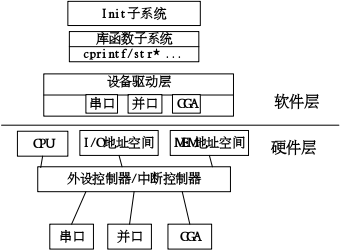
\includegraphics{figures/3.2.7.1.png}
\caption{3.2.7.1}
\end{figure}

在PC中的地址空间布局图如下所示:

\begin{figure}[htbp]
\centering
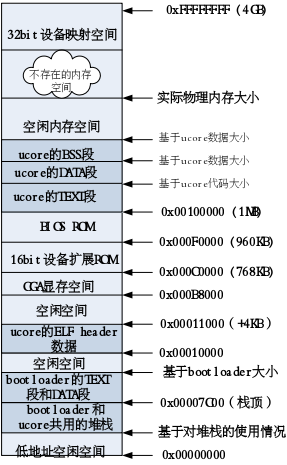
\includegraphics{figures/3.2.7.2.png}
\caption{3.2.7.2}
\end{figure}


\section{可管理中断并处理中断方式I/O的ucore}\label{ux53efux7ba1ux7406ux4e2dux65adux5e76ux5904ux7406ux4e2dux65adux65b9ux5f0fioux7684ucore}

\subsection{实验目标}\label{ux5b9eux9a8cux76eeux6807}

前面的project都没有引入中断机制,所以bootloader和ucore都是正常地顺序执行,不会受到外界(比如外设)的``干扰''。虽然实现简单,但无法解决上述问题。我们需要扩展ucore的功能,让ucore能够支持中断,这需要读者了解基本的80386硬件中断机制,对保护模式有更深入的了解;需要清楚在中断的处理过程中,硬件主动完成了什么事情,软件在硬件完成的基础上又要完成哪些事情。通过学习和实践,读者可以了解清楚上述问题,并进一步知道通过操作系统的中断处理例程(Interrupt
Process Routine, IPR)完成设备请求处理的方法等。

\subsection{proj4概述}\label{proj4ux6982ux8ff0}

\subsubsection{实现描述}\label{ux5b9eux73b0ux63cfux8ff0}

proj4建立在proj3.1的基础上,实现了一个通过中断机制完成设备(键盘、串口和时钟)中断请求处理的ucore。简单地说proj4扩展与中断相关的工作有两个,一个是初始化中断,涉及初始化中断控制器8259A(打通外设与CPU的通路)和中断门描述符表(建立外设中断与中断服务例程的联系)和各种外设。以proj4的ucore为例,操作系统内核启动以后,kern\_init函数(kern/init/init.c)通过调用pic\_init函数完成对中断控制器的初始化工作,调用idt\_init函数完成了对整个中断门描述符表的创建,调用cons\_init和clock\_init函数完成对串口、键盘和时钟外设的中断初始化工作。

ucore的另一个重要工作是中断服务,即收到中断后,对中断进行处理的中断服务例程(比如收到100个时钟中断后,显示一个字符串``100
ticks'')等。这主要集中在vectors.S(包括256个中断服务例程的入口地址和第一步初步处理实现)、trapentry.S(紧接着第一步初步处理后,进一步完成第二步初步处理的实现以及中断处理完毕后的返回准备工作)和trap.c中(紧接着第二步初步处理后,继续完成具体的各种中断处理操作)。

\subsubsection{项目组成}\label{ux9879ux76eeux7ec4ux6210}

proj4整体目录结构如下所示:

\begin{lstlisting}
proj4
|-- kern
|   |-- driver
|   |   |-- clock.c
|   |   |-- clock.h
|   |   |-- console.c
|   |   |-- console.h
|   |   |-- picirq.c
|   |   `-- picirq.h
|   |-- init
|   |   `-- init.c
|   |-- mm
|   |   |-- memlayout.h
|   |   `-- mmu.h
|   `-- trap
|       |-- trap.c
|       |-- trapentry.S
|       |-- trap.h
|       `-- vectors.S
`-- tools
    `-- vector.c
…… 
\end{lstlisting}

proj4是基于proj3.1(会在内置监控自身运行状态的ucore一节中进一步说明)进一步扩展完成的。相对于proj3.1,增加了大约10个文件,相关增加和改动主要集中在kern/driver和kern/trap目录下,使得ucore具有外设中断处理功能,这一个比较大的跨越。主要增加和修改的文件如下所示:

\begin{itemize}
\tightlist
\item
  tools/vector.c:生成vectors.S,此文件包含了中断向量处理的统一实现。
\item
  kern/driver/intr.{[}ch{]}:实现了通过设置CPU的eflags来屏蔽和使能中断的函数;
\item
  kern/driver/picirq.{[}ch{]}:实现了对中断控制器8259A的初始化和使能操作;
\item
  kern/driver/clock.{[}ch{]}:实现了对时钟控制器8253的初始化操作;
\item
  kern/driver/console.{[}ch{]}:实现了对串口和键盘的中断方式的处理操作;
\item
  kern/trap/vectors.S:包括256个中断服务例程的入口地址和第一步初步处理实现;
\item
  kern/trap/trapentry.S:紧接着第一步初步处理后,进一步完成第二步初步处理;并且有恢复中断上下文的处理,即中断处理完毕后的返回准备工作;
\item
  kern/trap/trap.{[}ch{]}:紧接着第二步初步处理后,继续完成具体的各种中断处理操作;
\end{itemize}

\subsubsection{编译运行}\label{ux7f16ux8bd1ux8fd0ux884c}

\textbf{编译运行}

编译并运行proj4的命令如下:

\begin{lstlisting}
make
make qemu
\end{lstlisting}

则可以得到如下显示界面 

通过上图可以看到时钟中断已经能够正常相应,每隔100个时钟中断会显示一次``100
ticks''的信息。一个简单的显示信息的背后蕴藏着中断处理的复杂实现。下面我们将从中断基本概念、中断控制器、保护模式的中断处理机制等方面来分析上图中背后的东西。

\section{【背景】理解CPU对外设中断的硬件支持}\label{ux80ccux666fux7406ux89e3cpuux5bf9ux5916ux8bbeux4e2dux65adux7684ux786cux4ef6ux652fux6301}

操作系统需要对计算机系统中的各种外设进行管理,这就需要CPU和外设能够相互通信才行。一般外设的速度远慢于CPU的速度。如果让操作系统通过CPU``主动关心''外设的事件,即采用通常的轮询(polling)机制,则太浪费CPU资源了。所以需要操作系统和CPU能够一起提供某种机制,让外设在需要操作系统处理外设相关事件的时候,能够``主动通知''操作系统,即打断操作系统和应用的正常执行,让操作系统完成外设的相关处理,然后在恢复操作系统和应用的正常执行。在操作系统中,这种机制称为中断机制。中断机制给操作系统提供了处理意外情况的能力,同时它也是实现进程/线程抢占式调度的一个重要基石。但中断引入的不确定性和异步性导致了设计和实现操作系统更加困难。

本章只描述保护模式下的中断处理过程。当CPU收到外设中断(可通过可编程中断控制器芯片8259A发给CPU中断信息)、CPU自身产生的故障(Fault)或CPU自身``有意''产生的陷阱(trap)时,它会暂停执行当前的程序或任务,通过一定的机制跳转到负责处理这个事件的相关处理例程中,在完成对这个事件的处理后再跳回到刚才被打断的程序或任务中。中断向量和中断服务例程的对应关系主要是由IDT(中断门描述符表)来描述。操作系统在IDT中设置好各种中断向量对应的中断描述符,而中断描述符指出了中断服务例程的起始地址,留待CPU在产生中断后查询对应中断服务例程的起始地址。而IDT本身的起始地址保存在IDTR寄存器中。

80386共支持256种中断,其中故障(Fault)和陷阱(Trap)由CPU自身产生,不使用中断控制器,也不能被屏蔽。外设中断又分为可屏蔽中断(INTR)和非屏蔽中断(NMI),I/O设备产生的中断请求(IRQ)引起可屏蔽中断,而紧急的外设事件(如掉电故障)引起的中断事件引起非屏蔽中断。

非屏蔽中断和异常的编号是固定的,而屏蔽中断的编号可以通过对中断控制器的编程来调整。256个中断的分配如下:
* 0\textsubscript{31号的中断对应于故障、陷阱和非屏蔽外设中断。 *
32}47号的中断分配给可屏蔽外设中断。 *
48\textasciitilde{}255号的中断可以用软件来设置。比如ucore可用其中的一个中断号来实现系统调用。

\subsection{外设可屏蔽中断}\label{ux5916ux8bbeux53efux5c4fux853dux4e2dux65ad}

80386通过两片中断控制器8259A来响应15个外中断源,每个8259A可管理8个中断源。第一级(称主片)的第二个中断请求输入端,与第二级8259A(称从片)的中断输出端INT相连,如下图所示。IRQ号和中断号之间的映射关系可以通过中断控制器来调整。

\begin{figure}[htbp]
\centering
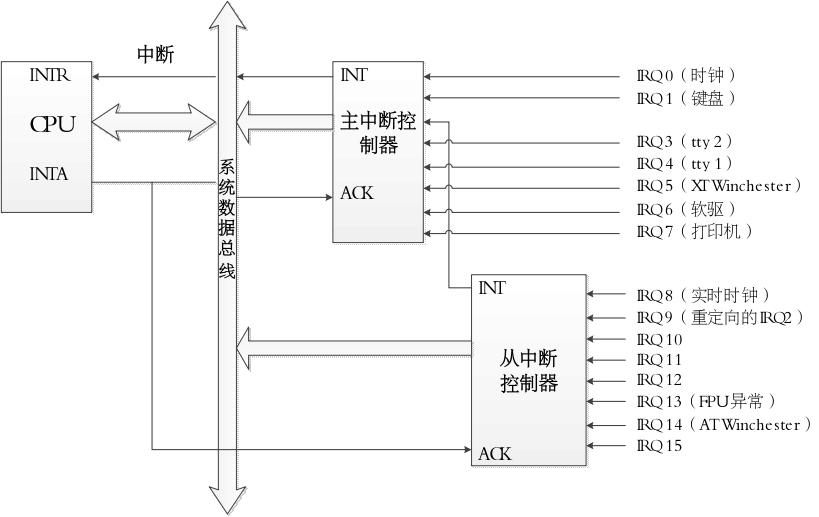
\includegraphics{figures/3.4.3.1.png}
\caption{3.4.3.1}
\end{figure}

级联的 8259A架构 \_\_\_

在中断产生过程中,中断控制器8259A监视外设产生的中断请求(IRQ)信号,如果外设产生了一个中断请求信号,则8259A执行如下操作:

\begin{enumerate}
\def\labelenumi{\arabic{enumi}.}
\item
  把接受到的IRQ信号转换成一个对应的中断编号;
\item
  把这个中断编号值存放在中断控制器的一个I/O地址单元中,CPU通过数据/地址总线可访问到此I/O地址单元;
\item
  给CPU的INTR引脚触发信号,即发出一个中断;
\item
  等待直到CPU通过INTA引脚确认这个中断信号,清除INTR引脚上的触发信号。
\end{enumerate}

屏蔽外部I/O请求有两种方法。一种是从CPU的角度清零CPU的EFLAG的中断标志位(IF);另一种是从中断控制器的角度,即通过把中断控制器中的中断屏蔽寄存器(IMR)相应位置1,则表示禁用某条中断线。

\subsection{陷阱、故障和非屏蔽中断}\label{ux9677ux9631ux6545ux969cux548cux975eux5c4fux853dux4e2dux65ad}

陷阱和故障是CPU内部执行指令的过程中产生的中断事件。非屏蔽中断就是计算机内部硬件出错时引起的紧急故障情况。80386处理器发布了大约20种陷阱、故障或非屏蔽中断。在某些故障产生时,CPU会产生一个硬件错误码并压入内核栈中。

在下表中给出了在实验中可能碰到的80386中陷阱的中断号、名称、类别及简单描述。更多的信息可以在Intel的技术文挡中找到。

表 ucore中异常的简单描述

\begin{lstlisting}
<td>中断号</td>
<td>名称</td>
<td>类别</td>
<td>简单描述</td>
\end{lstlisting}

\begin{lstlisting}
<td>8</td>
<td>双重故障</td>
<td>故障</td>
<td>在处理故障中又产生了故障</td>
\end{lstlisting}

\begin{lstlisting}
<td>11</td>
<td>段不存在</td>
<td>故障</td>
<td>访问一个不存在的段</td>
\end{lstlisting}

\begin{lstlisting}
<td>12</td>
<td>栈段异常</td>
<td>故障</td>
<td>超过栈段界限,或由ss标识的段不存在</td>
\end{lstlisting}

\begin{lstlisting}
<td>13</td>
<td>通用保护</td>
<td>故障</td>
<td>违反了保护模式下的某种保护规则</td>
\end{lstlisting}

\begin{lstlisting}
<td>14</td>
<td>页异常</td>
<td>故障</td>
<td>页不在内存,或违反了一种分页保护机制</td>
\end{lstlisting}

\subsection{中断门描述符表(Interrupt Descriptor
Table)}\label{ux4e2dux65adux95e8ux63cfux8ff0ux7b26ux8868interrupt-descriptor-table}

中断门描述符表把每个中断或异常编号和一个指向中断服务例程的描述符联系起来。同GDT一样,IDT是一个8字节的描述符数组,但IDT的第一项可以包含一个描述符。CPU把中断(异常)号乘以8做为IDT的索引。IDT可以位于内存的任意位置,CPU通过IDT寄存器(IDTR)的内容来寻址IDT的起始地址。指令LIDT和SIDT用来操作IDTR。两条指令都有一个显示的操作数:一个6字节表示的内存地址。指令的含义如下:
* LIDT(Load IDT
Register)指令:使用一个包含线性地址基址和界限的内存操作数来加载IDT。操作系统创建IDT时需要执行它来设定IDT的起始地址。这条指令只能在特权级0执行。
* SIDT(Store IDT
Register)指令:拷贝IDTR的基址和界限部分到一个内存地址。这条指令可以在任意特权级执行。

IDT和IDTR寄存器的结构和关系如下图所示:

\begin{figure}[htbp]
\centering
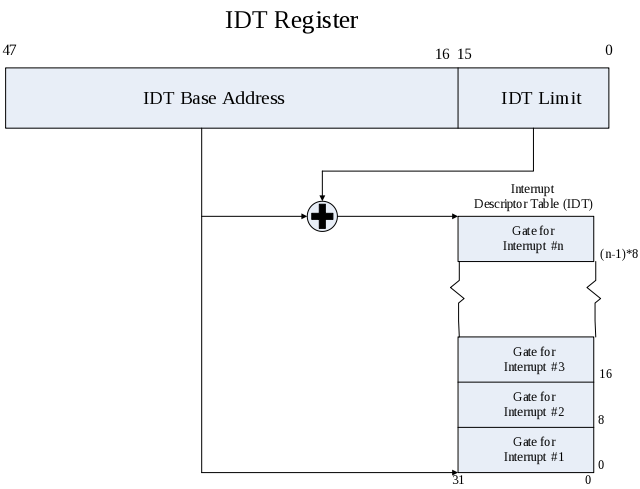
\includegraphics{figures/3.4.3.2.png}
\caption{3.4.3.2}
\end{figure}

在保护模式下,最多会存在256个Interrupt/Exception
Vectors。范围{[}0,31{]}内的32个向量被故障中断和NMI(不可屏蔽)中断使用,但当前并非所有这32个向量都已经被使用,有几个当前没有被使用。范围{[}32,255{]}内的向量被保留给用户定义的中断,可将它们用作外部I/O设备中断(8259A
IRQ),或者系统调用(System Call 、Software Interrupts)等。~

\subsection{门描述符(Gate
Descriptors)}\label{ux95e8ux63cfux8ff0ux7b26gate-descriptors}

在保护模式下,中断门描述符表(IDT)中的每个表项由8个字节组成,其中的每个表项叫做一个门描述符(Gate
Descriptor),
``门''的含义是指当中断发生时必须先访问这些``门'',能够``开门''(即将要进行的处理需通过特权检查,符合设定的权限等约束)后,然后才能进入相应的处理程序。而门描述符则描述了``门''的属性(如特权级、段内偏移量等)。在IDT中,可以包含如下3种类型的系统段描述符:

\begin{itemize}
\item
  中断门描述符(Interrupt-gate descriptor):
  用于中断处理,其类型码为110,中断门包含了一个外设中断或故障中断的处理程序所在段的选择子和段内偏移量。当控制权通过中断门进入中断处理程序时,处理器清IF标志,即关中断,以避免嵌套中断的发生。中断门中的DPL(Descriptor
  Privilege
  Level)为0,因此用户态的进程不能访问中断门。所有的中断处理程序都由中断门激活,并全部限制在内核态。
\item
  陷阱门描述符(Trap-gate
  descriptor):用于系统调用,其类型码为111,与中断门类似,其唯一的区别是,控制权通过陷阱门进入处理程序时维持IF标志位不变,也就是说,不关中断。
\item
  任务门描述符(Task-gate descriptor)和调用门描述符(Call-gate
  descriptor):
  这两种主要是Intel设置的``任务''切换的手段,在本书中暂时没有使用。
\end{itemize}

下图图显示了80386的中断门描述符、陷阱门描述符的格式:

\begin{figure}[htbp]
\centering
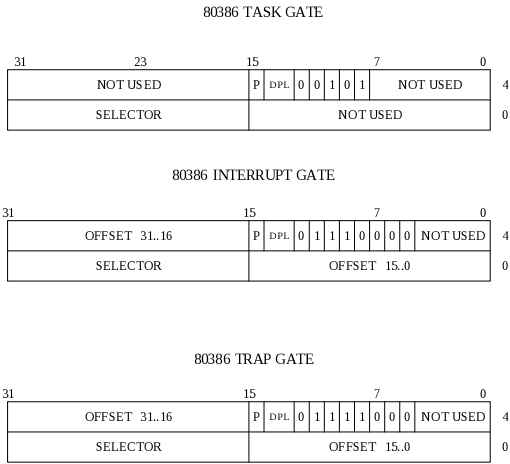
\includegraphics{figures/3.4.3.3.png}
\caption{3.4.3.3}
\end{figure}

\subsection{中断处理中硬件负责完成的工作}\label{ux4e2dux65adux5904ux7406ux4e2dux786cux4ef6ux8d1fux8d23ux5b8cux6210ux7684ux5de5ux4f5c}

中断服务例程包括具体负责处理中断(异常)的代码是操作系统的重要组成部分。需要注意区别的是,有两个过程由硬件完成:
*
硬件中断处理过程1(起始):从CPU收到中断事件后,打断当前程序或任务的执行,根据某种机制跳转到中断服务例程去执行的过程。其具体流程如下:

\begin{lstlisting}
1. CPU在执行完当前程序的每一条指令后,都会去确认在执行刚才的指令过程中中断控制器(如8259A)是否发送中断请求过来,如果有那么CPU就会在相应的时钟脉冲到来时从总线上读取中断请求对应的中断向量;
2. CPU根据得到的中断向量(以此为索引)到IDT中找到该向量对应的中断描述符,中断描述符里保存着中断服务例程的段选择子;
3. CPU使用IDT查到的中断服务例程的段选择子从GDT中取得相应的段描述符,段描述符里保存了中断服务例程的段基址和属性信息,段描述符的基址+中断描述符中的偏移地址形成了中断服务例程的起始地址;
4. CPU会根据CPL和中断服务例程的段描述符的DPL信息确认是否发生了特权级的转换。比如当前应用程序正运行在用户态,而中断服务例程是运行在内核态的,则意味着发生了特权级的转换,这时CPU会从当前应用程序的TSS信息(该信息在内存中的起始地址存在TR寄存器中)里取得该程序的内核栈地址,即包括内核态的ss和esp的值,并立即将系统当前使用的栈切换成新的内核栈。这个栈就是即将运行的中断服务程序要使用的栈。紧接着就将当前程序使用的用户态的ss和esp压到新的内核栈中保存起来;如果当前程序运行在内核态,则不会发生特权转移
5. CPU需要开始保存当前被打断的用户态程序的现场(即一些寄存器的值),以便于将来恢复被打断的程序继续执行。这需要利用内核栈来保存相关现场信息,即依次压入当前被打断程序使用的eflags,cs,eip,errorCode(如果是有错误码的异常)信息;
6. CPU把中断服务例程的地址加载到cs和eip寄存器中,开始执行中断服务例程。这意味着先前的程序被暂停执行,中断服务程序正式开始工作。
\end{lstlisting}

\begin{itemize}
\item
  硬件中断处理过程2(结束):每个中断服务例程在有中断处理工作完成后需要通过iret(或iretd)指令恢复被打断的程序的执行。CPU执行IRET指令的具体过程如下:

  \begin{enumerate}
  \def\labelenumi{\arabic{enumi}.}
  \item
    程序执行这条iret指令时,首先会从内核栈里弹出先前保存的被打断的程序的现场信息,即eflags,cs,eip重新开始执行;
  \item
    如果存在特权级转换(从内核态转换到用户态),则还需要从内核栈中弹出用户态栈的ss和esp,这样也意味着栈也被切换回原先使用的用户态的栈了;
  \item
    如果此次处理的是带有错误码(errorCode)的异常,CPU在恢复先前程序的现场时,并不会弹出errorCode。这一步需要通过软件完成,即要求相关的中断服务例程在调用iret返回之前添加出栈代码主动弹出errorCode。
  \end{enumerate}
\end{itemize}

下图显示了从中断向量到GDT中相应中断服务程序起始位置的定位方式:

\begin{figure}[htbp]
\centering
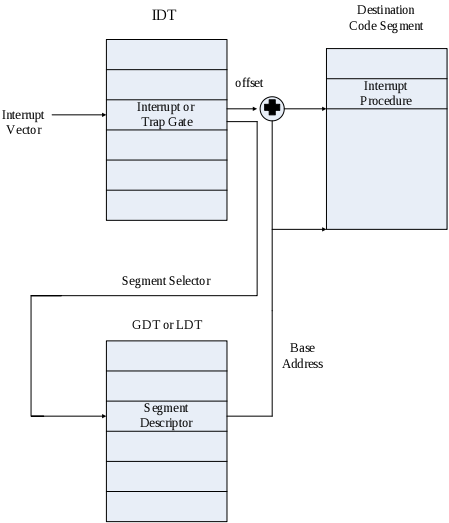
\includegraphics{figures/3.4.3.4.png}
\caption{3.4.3.4}
\end{figure}

\subsection{中断处理的特权级转换}\label{ux4e2dux65adux5904ux7406ux7684ux7279ux6743ux7ea7ux8f6cux6362}

中断处理得特权级转换是通过门描述符(gate
descriptor)和相关指令来完成的。一个门描述符就是一个系统类型的段描述符,一共有4个子类型:调用门描述符(call-gate
descriptor),中断门描述符(interrupt-gate
descriptor),陷阱门描述符(trap-gate
descriptor)和任务门描述符(task-gate
descriptor)。与中断处理相关的是中断门描述符和陷阱门描述符。这些门描述符被存储在中断门描述符表(Interrupt
Descriptor
Table,简称IDT)当中。CPU把中断向量作为IDT表项的索引,用来指出当中断发生时使用哪一个门描述符来处理中断。中断门描述符和陷阱门描述符几乎是一样的。中断发生时实施特权检查的过程如下图所示:

\begin{figure}[htbp]
\centering
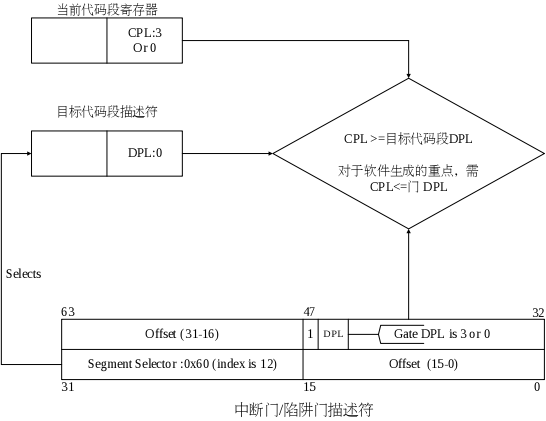
\includegraphics{figures/3.4.3.5.png}
\caption{3.4.3.5}
\end{figure}

图 中断发生时实施特权检查的过程

门中的DPL和段选择符一起控制着访问,同时,段选择符结合偏移量(Offset)指出了中断处理例程的入口点。内核一般在门描述符中填入内核代码段的段选择子。产生中断后,CPU一定不会将运行控制从高特权级转向低特权级,特权级必须要么保持不变(当操作系统内核自己被中断的时候),或被提升(当用户态程序被中断的时候)。无论哪一种情况,作为结果的CPL必须等于目的代码段的DPL。如果CPL发生了改变(比如从用户态到内核态),一个栈切换操作(通过TSS完成)就会发生。如果中断是被用户态程序中的指令所触发的(比如软件执行INT
n生产的中断),还会增加一个额外的检查:门的DPL必须具有与CPL相同或更低的特权。这就防止了用户代码随意触发中断。如果这些检查失败,就会产生一个一般保护异常(general-protection
exception)。

\section{【实现】初始化中断控制器}\label{ux5b9eux73b0ux521dux59cbux5316ux4e2dux65adux63a7ux5236ux5668}

80386把中断号0~31分配给陷阱、故障和非屏蔽中断,而把32~47之间的中断号分配给可屏蔽中断。可屏蔽中断的中断号是通过对中断控制器的编程来设置的。下面描述了对8259A中断控制器初始化过程。

8259A通过两个I/O地址来进行中断相关的数据传送,对于单个的8259A或者是两级级联中的主8259A而言,这两个I/O地址是0x20和0x21。对于两级级联的从8259A而言,这两个I/O地址是0xA0和0xA1。8259A有两种编程方式,一是初始化方式,二是工作方式。在操作系统启动时,需要对8959A做一些初始化工作,即实现8259A的初始化方式编程。8259A中的四个中断命令字(ICW)寄存器用来完成初始化编程,其含义如下:

\begin{itemize}
\item
  ICW1:初始化命令字。
\item
  ICW2:中断向量寄存器,初始化时写入高五位作为中断向量的高五位,然后在中断响应时由8259根据中断源(哪个管脚)自动填入形成完整的8位中断向量(或叫中断类型号)。
\item
  ICW3: 8259的级联命令字,用来区分主片和从片。
\item
  ICW4:指定中断嵌套方式、数据缓冲选择、中断结束方式和CPU类型。
\end{itemize}

8259A初始化的过程就是写入相关的命令字,8259A内部储存这些命令字,以控制8259A工作。有关的硬件可看附录补充资料。这里只把ucore对8259A的初始化过程(在picirq.c中的pic\_init函数实现)描述一下:

\begin{lstlisting}
//此时系统尚未初始化完毕,故屏蔽主从8259A的所有中断

outb(IO_PIC1 + 1, 0xFF);
outb(IO_PIC2 + 1, 0xFF);

// 设置主8259A的ICW1,给ICW1写入0x11,0x11表示(1)外部中断请求信号为上升沿触发有效,(2)系统中有多片8295A级联,(3)还表示要向ICW4送数据

// ICW1设置格式为:  0001g0hi  
//    g:  0 = edge triggering, 1 = level triggering  
//    h:  0 = cascaded PICs, 1 = master only  
//    i:  0 = no ICW4, 1 = ICW4 required  

outb(IO_PIC1, 0x11);

// 设置主8259A的ICW2:  给ICW2写入0x20,设置中断向量偏移值为0x20,即把主8259A的IRQ0-7映射到向量0x20-0x27

outb(IO_PIC1 + 1, IRQ_OFFSET);

// 设置主8259A的ICW3:  ICW3是8259A的级联命令字,给ICW3写入0x4,0x4表示此主中断控制器的第2个IR线(从0开始计数)连接从中断控制器。

outb(IO_PIC1 + 1, 1 << IRQ_SLAVE);

//设置主8259A的ICW4:给ICW4写入0x3,0x3表示采用自动EOI方式,即在中断响应时,在8259A送出中断矢量后,自动将ISR相应位复位;并且采用一般嵌套方式,即当某个中断正在服务时,本级中断及更低级的中断都被屏蔽,只有更高的中断才能响应。

// ICW4设置格式为:  000nbmap
//    n:  1 = special fully nested mode
//    b:  1 = buffered mode
//    m:  0 = slave PIC, 1 = master PIC
//      (ignored when b is 0, as the master/slave role
//      can be hardwired).
//    a:  1 = Automatic EOI mode
//    p:  0 = MCS-80/85 mode, 1 = intel x86 mode
outb(IO_PIC1 + 1, 0x3);

//设置从8259A的ICW1:含义同上

outb(IO_PIC2, 0x11);    // ICW1

//设置从8259A的ICW2:给ICW2写入0x28,设置从8259A的中断向量偏移值为0x28

outb(IO_PIC2 + 1, IRQ_OFFSET + 8);  // ICW2

//0x2表示此从中断控制器链接主中断控制器的第2个IR线

outb(IO_PIC2 + 1, IRQ_SLAVE);   // ICW3

//设置主8259A的ICW4:含义同上

outb(IO_PIC2 + 1, 0x3); // ICW4

//设置主从8259A的OCW3:即设置特定屏蔽位(值和英文解释不一致),允许中断嵌套;不查询;将读入其中断请求寄存器IRR的内容

// OCW3设置格式为:  0ef01prs
//   ef:  0x = NOP, 10 = clear specific mask, 11 = set specific mask
//    p:  0 = no polling, 1 = polling mode
//   rs:  0x = NOP, 10 = read IRR, 11 = read ISR
outb(IO_PIC1, 0x68);    // clear specific mask
outb(IO_PIC1, 0x0a);    // read IRR by default

outb(IO_PIC2, 0x68);    // OCW3
outb(IO_PIC2, 0x0a);    // OCW3

//初始化完毕,使能主从8259A的所有中断

if (irq_mask != 0xFFFF) {
    pic_setmask(irq_mask);
}
\end{lstlisting}


\section{【实现】初始化中断门描述符表}\label{ux5b9eux73b0ux521dux59cbux5316ux4e2dux65adux95e8ux63cfux8ff0ux7b26ux8868}

ucore操作系统如果要正确处理各种不同的中断事件,就需要安排应该由哪个中断服务例程负责处理特定的中断事件。系统将所有的中断事件统一进行了编号(0~255),这个编号称为中断号或中断向量。

为了完成中断号和中断服务例程起始地址的对应关系,首先需要建立256个中断处理例程的入口地址。为此,通过一个
C程序 tools/vector.c 生成了一个文件vectors.S,在此文件中的
\_\_vectors地址处开始处连续存储了256个中断处理例程的入口地址数组,且在此文件中的每个中断处理例程的入口地址处,实现了中断处理过程的第一步初步处理。

有了中断服务例程的起始地址,就可以建立对应关系了,这部分的实现在trap.c文件中的idt\_init函数中实现:

\begin{lstlisting}
//全局变量:中断门描述符表

static struct gatedesc idt[256] = {{0}};
……
void idt_init(void) {

//保存在vectors.S中的256个中断处理例程的入口地址数组

    extern uint32_t __vectors[];
    int i;
  
//在中断门描述符表中通过建立中断门描述符,其中存储了中断处理例程的代码段GD_KTEXT和偏移量\__vectors[i],特权级为DPL_KERNEL。这样通过查询idt[i]就可定位到中断服务例程的起始地址。

    for (i = 0; i < sizeof(idt) / sizeof(struct gatedesc); i ++) {
        SETGATE(idt[i], 0, GD_KTEXT, __vectors[i], DPL_KERNEL);
    }
  
//建立好中断门描述符表后,通过指令lidt把中断门描述符表的起始地址装入IDTR寄存器中,从而完成中段描述符表的初始化工作。

    lidt(&idt_pd);
}
\end{lstlisting}


\section{【实现】外设的相关中断初始化}\label{ux5b9eux73b0ux5916ux8bbeux7684ux76f8ux5173ux4e2dux65adux521dux59cbux5316}

串口的初始化函数serial\_init(位于/kern/driver/console.c)中涉及中断初始化工作的很简单:

\begin{lstlisting}
......
// 使能串口1接收字符后产生中断
    outb(COM1 + COM_IER, COM_IER_RDI);
......
// 通过中断控制器使能串口1中断
pic_enable(IRQ_COM1);
\end{lstlisting}

键盘的初始化函数kbd\_init(位于kern/driver/console.c中)完成了对键盘的中断初始化工作,具体操作更加简单:

\begin{lstlisting}
......
// 通过中断控制器使能键盘输入中断
pic_enable(IRQ_KBD);
\end{lstlisting}

时钟是一种有着特殊作用的外设,其作用并不仅仅是计时。在后续章节中将讲到,正是由于有了规律的时钟中断,才使得无论当前CPU运行在哪里,操作系统都可以在预先确定的时间点上获得CPU控制权。这样当一个应用程序运行了一定时间后,操作系统会通过时钟中断获得CPU控制权,并可把CPU资源让给更需要CPU的其他应用程序。时钟的初始化函数clock\_init(位于kern/driver/clock.c中)完成了对时钟控制器8253的初始化:

\begin{lstlisting}
    ......
//设置时钟每秒中断100次
    outb(IO_TIMER1, TIMER_DIV(100) % 256);
    outb(IO_TIMER1, TIMER_DIV(100) / 256);
// 通过中断控制器使能时钟中断
    pic_enable(IRQ_TIMER);
\end{lstlisting}


\section{【实现】中断处理过程}\label{ux5b9eux73b0ux4e2dux65adux5904ux7406ux8fc7ux7a0b}

当中断产生后,首先硬件要完成一系列的工作(如小节``中断处理中硬件负责完成的工作''所描述的``硬件中断处理过程1(起始)''内容),由于中断发生在内核态执行过程中,所以特权级没有变化,所以CPU在跳转到中断处理例程之前,还会在内核栈中依次压入错误码(可选)、EIP、CS和EFLAGS,下图显示了在相同特权级下中断产生后的栈变化示意图:

\begin{figure}[htbp]
\centering
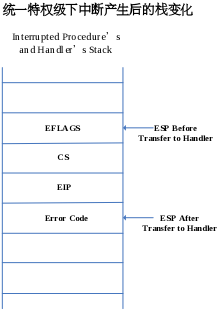
\includegraphics{figures/3.4.7.1.png}
\caption{3.4.7.1}
\end{figure}

然后CPU就跳转到IDT中记录的中断号i所对应的中断服务例程入口地址处继续执行。
vector.S 文件中定义了每个中断的中断处理例程的入口地址 (保存在 vectors
数组中)。其中,中断可以分成两类:一类是压入错误编码的 (error
code),另一类不压入错误编码。对于第二类, vector.S 自动压入一个
0。此外,还会压入相应中断的中断号。在内核栈中压入一个或两个必要的参数之后,都会跳转到统一的入口
\_\_alltraps 处(位于trapentry.S中)继续执行。

CPU从\_\_alltraps处开始,在栈中按照trapframe结构压入各个寄存器,此时内核栈的结构如下所示:

\begin{lstlisting}
uint32_t reg_edi;
uint32_t reg_esi;
uint32_t reg_ebp;
uint32_t reg_oesp;          /* Useless */
uint32_t reg_ebx;
uint32_t reg_edx;
uint32_t reg_ecx;
uint32_t reg_eax;   
uint16_t tf_es;
uint16_t tf_padding1;
uint16_t tf_ds;
uint16_t tf_padding2;
uint32_t tf_trapno;
/* below here defined by x86 hardware */
uint32_t tf_err;
uintptr_t tf_eip;
uint16_t tf_cs;
uint16_t tf_padding3;
uint32_t tf_eflags;
\end{lstlisting}

此时,为了将来能够恢复被打断的内核执行过程所需的寄存器内容都保存好了。为了正确进行中断处理,把DS和ES寄存器设置为GD\_KDATA,这是为了预防从用户态产生的中断(当然,到目前为止,ucore都在内核态执行,还不会发生这种情况)。把刚才保存的trapframe结构的起始地址(即当前SP值)压栈,然后调用
trap函数(定义在trap.c中),就开始了对具体中断的处理。trap进一步调用trap\_dispatch函数,完成对具体中断的处理。在相应的处理过程结束以后,trap将会返回,在\_\_trapret:中,完成对返回前的寄存器和栈的回复准备工作,最后通过iret指令返回到中断打断的地方继续执行。整个中断处理流程大致如下:

\begin{figure}[htbp]
\centering
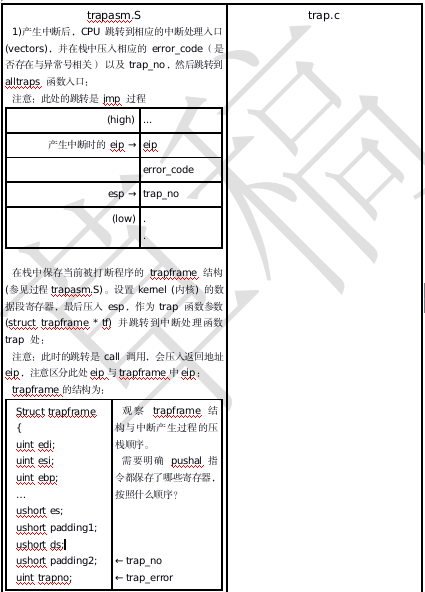
\includegraphics{figures/3.4.7.2.png}
\caption{3.4.7.2}
\end{figure}

\begin{figure}[htbp]
\centering
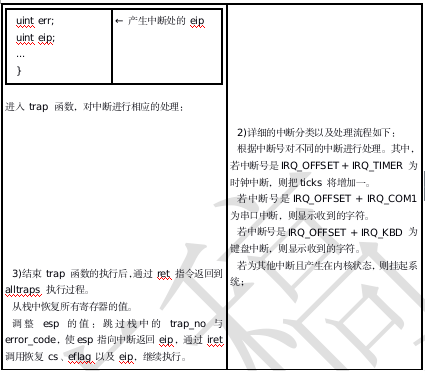
\includegraphics{figures/3.4.7.3.png}
\caption{3.4.7.3}
\end{figure}


\section{小结}
缺